\documentclass[runningheads]{llncs}

\usepackage[T1]{fontenc}
\usepackage{graphicx}
\usepackage{amsmath}
\usepackage{booktabs}
\usepackage{longtable}
\usepackage{tabularx}
\usepackage{array}
\usepackage{hyperref}

\newcolumntype{Y}{>{\raggedright\arraybackslash}X}
\hypersetup{hidelinks}

\begin{document}

\title{A Governed Public-Data Benchmark of Quantum Machine Learning for Human-Rated Cislunar Trajectory-Correction Planning}
\titlerunning{A Governed QML Benchmark for Cislunar Trajectory Correction}

\author{Taechasith Kangkhuntod}
\authorrunning{T. Kangkhuntod}
\institute{University of the Thai Chamber of Commerce, Bangkok, Thailand}

\maketitle

\begin{abstract}
This research asks whether quantum-kernel models add predictive value to a
public-data, human-rated cislunar trajectory-correction decision-support
benchmark when compared fairly with physics-based controls. The
study froze its source-bound simulator, grouped development splits, fold-local
preprocessing, retention rules, and claim boundary before model outcomes were
reported. The simulator credibility chain accepted 67 eligible public-data
checks with zero failures. The preregistered Q01 fidelity-style quantum kernel
had mean normalized root-mean-square error (NRMSE) 0.646614, compared with
0.008739 for the C06 physics-residual control; no regime qualified for advance.
The projected Q01b successor had NRMSE 0.661207 versus 0.006833 for C06. A
feasibility-only quantum kernel reached recall 0.108860 at the frozen threshold,
which was inadequate for its safety-filter interpretation. Sixteen further,
prospectively bounded development-only candidates completed as valid negatives;
the strongest apparent residual gain did not survive its matched classical
control. The finding is not that QML is universally ineffective. It is that the
tested QML representations did not justify additional complexity for this
frozen task and control set. The societal contribution is a transparent method
for preventing unsupported AI claims from being promoted into high-consequence
human decision contexts: preserve source provenance, show negative outcomes,
and keep crew-related requirements and human review separate from a model score.
This study does not claim quantum advantage, propellant savings, mission-loop
validity, flight readiness, hardware performance, or a new QML invention.
\keywords{Quantum machine learning \and human-centered AI \and decision support \and cislunar trajectory design \and reproducible benchmarking \and negative results}
\end{abstract}

\section{Introduction}

Cislunar space is the region in and around the Earth--Moon system. A
trajectory-correction maneuver, or correction burn, deliberately changes a
spacecraft's velocity to keep its path within mission constraints. The required
change is summarized by delta-v (measured in m/s). Delta-v is not propellant
mass, although it is a standard measure of maneuver effort and is related to
fuel use through the vehicle and propulsion model.

For a crew-carrying mission, correction planning is a coupled decision problem:
burn timing and delta-v interact with navigation uncertainty, maneuver
execution, crew timelines, entry conditions, and reserve constraints. Public
Artemis trajectory-design research therefore treats robust correction cost,
meaning correction delta-v evaluated with modeled uncertainty, together with
mission constraints rather than as an unconstrained curve-fitting task
\cite{woffinden2023}. A learning \emph{surrogate}, a fast predictive model that
approximates a more expensive simulation, could help screen candidate scenarios.
That possibility is a motivation for testing, not evidence that a particular
machine-learning model is useful or safe.

The paper adopts a human-centered decision-support framing. A model score is
not the decision: a responsible reviewer needs to know which source data,
physical assumptions, uncertainty boundary, and failure cases produced the
score before deciding whether a model warrants further study. Crew-related
requirements therefore remain separate from predictive performance, consistent
with the intended-use and human-system boundaries in the applicable U.S.
National Aeronautics and Space Administration (NASA) standards
\cite{nasa7009,nasa3001}. This work does not conduct a user study or measure
usability, trust, workload, or operator performance. From a human--computer
interaction (HCI) perspective, its contribution is the evidence design around
a possible future decision-support tool.

Quantum machine learning (QML) uses quantum-state representations or quantum
circuits inside a learning method. In a quantum-kernel model, a circuit maps
each classical input to a quantum state and the overlap between two states is
used as a similarity score. This offers feature maps different from common
classical models \cite{schuld2019,havlicek2019}, but difference alone does not
imply usefulness. Encoding data introduces loading choices, similarity
geometry, and resource costs. A circuit may be difficult to simulate in general
while still being approximated well by a classical learner on the tested data
\cite{huang2021,sweke2025}. Conversely, a favorable result can arise from a
weakly tuned comparator, related mission cases leaking across a data split,
thresholds chosen after seeing outcomes, or omitted failures. These are
benchmarking problems before they are quantum-computing problems.

This paper documents a complete public-data experimental program for
trajectory-correction prediction and feasibility screening. The purpose was
not to assert a priori that QML would win. Its purpose was to establish a
scientifically usable decision process: define a bounded task, verify the
simulator against eligible public endpoints, freeze the development protocol,
compare QML with strong controls, record negative outcomes, and prohibit
claims that the evidence cannot support. This stance is consistent with model
and simulation credibility practice \cite{nasa7009} and with recent calls for
fair QML comparisons \cite{bowles2024,schnabel2024}.

The central research questions were deliberately narrow:
\begin{enumerate}
\item Can the primary fidelity-style quantum kernel (repository identifier
Q01) improve correction-cost prediction over physics-derived and classical
controls under the frozen development protocol?
\item If Q01 fails, can the projected follow-up Q01b improve the same task
without changing data access or data splits?
\item Can the feasibility-only quantum kernel (FQK) meet its fixed screening
criteria for identifying independently propagated feasible cases?
\item Which conclusions remain valid when calibration, final-test,
mission-loop, and hardware evidence stay locked?
\end{enumerate}

The answer to the first three questions is negative for the tested models and
settings. The fourth question is the paper's main methodological contribution.
The work establishes a transparent evidence hierarchy that distinguishes
simulator credibility, development-only model evidence, future-design lessons,
and prohibited operational claims. Negative results are not treated as failed
record keeping; they are the result when a hypothesis does not meet its
predeclared standard.

The paper makes six contributions:
\begin{enumerate}
\item A source-bound cislunar benchmark protocol, meaning that inputs are tied
to identified public files and recorded source versions, with grouped
development folds, training-fold-only transformations, and retained numerical
feasibility outcomes.
\item A simulator credibility chain that reports its eligible scope and its
source-ineligible exception rather than converting missing evidence into a
pass or failure.
\item A preregistered QML comparison against physics-residual, random-feature,
compressed-input, and classical kernel controls.
\item A closed successor ledger containing exploratory and prospectively
bounded negative candidates, including classical controls that replace the
quantum component while keeping the surrounding construction matched.
\item A self-contained evidence and figure package that supports review of the
negative conclusion without widening the study's scientific claim.
\item A human-centered claim boundary that keeps model evidence, crew-related
requirements, and future human authorization distinct.
\end{enumerate}

\section{Scientific Scope and Claim Boundary}
\label{sec:scope}

The study is an offline, public-data, development-only benchmark. It is not a
mission design authority, a flight certification exercise, or a performance
assessment of a quantum processor. A simulation result may be useful for
evaluating a model family, but it cannot by itself establish the performance
of a mission-owned trajectory system or a hardware quantum implementation.
The distinction is essential for a human-rated application, where human-system
requirements are separate from a surrogate's regression score
\cite{nasa3001}.

\subsection{Reader guide to labels and data stages}

Short identifiers are retained because they link the paper to immutable
repository records. They are audit keys, not scientific concepts that a reader
is expected to know in advance:
\begin{description}
\item[Gate.] A predefined authorization checkpoint. Gate 3 asks whether the
simulator is credible within its public-data scope; Gate 5 evaluates models on
development data; Gate 6 would be a separately authorized mission-level
experiment and was never opened.
\item[Decision and protocol IDs.] A label beginning with D identifies a
governance decision or bounded campaign, while P identifies a prospective
protocol. For example, D046 is the decision record for one successor test.
These labels are not data samples or performance grades.
\item[Model IDs.] C labels a classical candidate, Q labels a QML candidate,
and A labels an analysis control. Thus C06 is the physics-residual classical
control and Q01 is the primary quantum-kernel candidate.
\item[Figure IDs.] RFIG identifies the repository's provenance record for a
figure. It allows the plotted data and generating script to be found; it has no
statistical meaning.
\item[Development-only.] Development rows may be used to choose and compare
models. Calibration rows would adjust a frozen model's output, and final-test
rows would estimate performance only after all choices were fixed. This study
read neither calibration nor final-test rows for the reported campaigns.
\item[Fold, seed, and rung.] A fold is one group-preserving train/validation
partition. A seed is a fixed random-number starting point used to repeat a
model reproducibly. A rung is one sample-size stage in the prespecified
128--1,024-row screening sequence.
\end{description}

\subsection{Human-centered decision-support stance}

The proposed role of a model in this benchmark is limited to offline screening
information for qualified human review. It is not an autonomous controller,
an operational recommendation engine, or a replacement for mission analysis.
For an HCI-oriented reading, the central design requirements are traceability,
understandable scope, visible uncertainty, retained failures, and a clear
fallback to physical analysis. The evidence package supports those requirements
by showing the data boundary, simulator checks, controls, stopping decisions,
and excluded evidence pathways together with the metrics.

No human participants, operator interfaces, observational studies, or measures
of trust, workload, situation awareness, or decision quality were collected.
The paper therefore makes no empirical HCI performance claim. It instead
describes how a high-consequence AI research artifact can be structured so that
later human evaluation is not pre-empted by an unsupported model claim.

The evidence boundary was defined before reporting. Gate 3 supports simulator
credibility only for the eligible comparisons. Gate 5 supports a technical
decision for a frozen development benchmark. The subsequent projected-kernel
protocol (P001) and 16 bounded successor decisions (D034--D049) are
development-only follow-ups; they cannot retroactively change the Gate 5
decision. Calibration and final-test rows, mission-loop
scenarios, quantum-hardware or graphics-processor execution, threshold application to real
operations, trained-model release, and Gate 6 remain outside the study. Table
\ref{tab:claim-boundary} summarizes the resulting language constraints.

\begin{table}[t]
\caption{Claim boundary used throughout the manuscript. This table is derived from the committed claim-boundary record and does not add a new experimental result.}
\label{tab:claim-boundary}
\centering
\footnotesize
\begin{tabularx}{\textwidth}{@{}p{0.19\textwidth}X@{}}
\toprule
Evidence category & Permitted interpretation \\
\midrule
Gate 3: simulator credibility & Simulator agreement for eligible public-data checks, not flight validation. RTC3 lacked eligible post-event evidence, so it was not tested and is neither a pass nor a failure. \\
Gate 5: development benchmark & Under the frozen development benchmark, the tested QML candidates did not outperform strong classical controls. \\
Post-Gate follow-ups & Projected-kernel protocol P001 and successor decisions D034--D049 are development-only negatives. They do not revise Gate 5 or authorize Gate 6. \\
Screening lesson & The recall-first classical analysis is a future protocol-design lesson, not a deployed safety filter or safety result. \\
Prohibited claims & No quantum advantage, propellant saving, mission-loop validity, flight readiness, NASA approval, hardware behavior, final-test result, or QML invention claim. \\
\bottomrule
\end{tabularx}
\end{table}


Figure \ref{fig:timeline} records the governance state rather than a model
metric. It is included because a benchmark conclusion depends on which evidence
was authorized when. A later candidate may be scientifically informative, but
it does not become preregistered evidence merely because it is reported after a
negative primary result.

\begin{figure}[t]
\centering

\includegraphics[width=\textwidth]{figures/gate_decision_timeline.png}
\caption{Research governance through Gate 5 (RFIG-001). Gates 0--5 were
closed by human decisions; the technical Gate 5 result is a benchmark-specific
protocol FAIL, meaning its advancement hypothesis was rejected. Gate 6 remains
unopened. This is decision-state evidence, not a model
performance plot.}
\label{fig:timeline}
\end{figure}

\section{Related Work and Positioning}

The target problem is positioned relative to public work on Artemis
trajectory-correction design, rather than being presented as a replacement for
mission-owned analysis. Woffinden et al. describe a correction-burn placement
formulation that incorporates uncertainty, crew-related timing, and entry
constraints \cite{woffinden2023}. Classical learning research has explored
low-thrust guidance and cislunar transfer design, but those settings differ in
dynamics, propulsion, objectives, and validation structure
\cite{sullivan2021,izzo2021,xie2022}. They are valuable precedents for
surrogate modeling and for retaining infeasible cases, not interchangeable
baselines for a human-rated correction benchmark.

Quantum feature-space methods express a classical input through an encoding
and compare encoded states by a quantum-derived similarity
\cite{schuld2019,havlicek2019}. The method can be used in a kernel learner,
but its predictive value depends on an alignment between the data geometry,
the feature map, the measurement, and the task. Theoretical and numerical work
has made this caveat increasingly explicit: hard-to-simulate circuits do not
automatically give a learning advantage, and the data distribution can make a
classical approximation competitive \cite{huang2021,sweke2025}.

The present work is particularly informed by three benchmarking lessons. First,
kernel bandwidth and encoding scale are part of the effective inductive bias,
not negligible implementation details \cite{shaydulin2022}. Second, a
quantum-kernel study should include appropriately strong classical
counterparts, including random features where relevant
\cite{otten2020,sweke2025}. Third, a comparison should report more than its
best run: model choice, split structure, seed variation, capacity, and
post-outcome choices all affect what a claimed gain means
\cite{bowles2024,schnabel2024,pernot2020}.

This paper does not make an exhaustive literature-review claim. The repository
preserves a bounded extraction set of 23 accepted records used to establish the
initial protocol and a separate archival discovery refresh. The refresh did
not change the experiment, thresholds, figures, or outcomes. Literature is
therefore used here to position the benchmark and justify controls, not to
construct a retrospective theory of success.

\section{Materials and Methods}
\label{sec:methods}

\subsection{Scenario construction and simulator credibility}

The public pipeline generated correction scenarios at three frozen levels of
physical detail. F0 uses central Earth point-mass gravity. F1 adds the Moon and
Sun as third-body gravitational sources. F2 additionally includes Earth J2,
the leading correction for Earth's equatorial bulge, and tighter numerical
integration settings. Across these levels the implementation retained the
configured maneuver model, mass depletion, event handling, crew-related
constraints, uncertainty variables, and numerical feasibility checks. The
intent was to predict benchmark-defined cost or feasibility outcomes, not to
control a spacecraft. Source files and scenario construction were frozen before
the model campaigns; later reports could summarize outputs but could not
replace source evidence to make a comparison pass.

Simulator credibility was assessed in Gate 3 by comparing eligible Python
trajectory endpoints with NASA's General Mission Analysis Tool (GMAT) under
the same accepted force-model configurations. An endpoint is the simulated
position and velocity at the end of a validation window. The diagnostic chain
isolated a formatting problem in the file containing the Earth-J2 coefficient
and confirmed the repaired format through degree-two, order-zero gravity
comparisons. In the final accepted evidence, all 67 evaluable checks passed;
the repaired endpoint set also passed the unchanged position and velocity
limits. This supports the implementation only within the tested public scope;
it does not validate a complete mission environment.

One record, the third return-trajectory-correction event (RTC3), is explicitly
excluded from the claim. Its qualified public trajectory file was created
before the event and therefore cannot show the event's reconstructed outcome
under the frozen temporal-evidence rule. It is
therefore classified as \texttt{not\_eligible}, rather than as a successful
or failed endpoint. This distinction prevents an important category error:
source eligibility is not a numerical outcome. The exclusion remains visible
in the evidence package rather than being silently omitted.

\subsection{Frozen development data and leakage control}

Let $\mathcal{D}=\{(x_i,y_i,z_i,g_i)\}_{i=1}^{N}$ denote the frozen
development dataset, where $N$ is the total number of development rows and $i$
indexes one simulated candidate plan. The vector $x_i$ contains only the
allowed scenario features. The target $y_i$ is robust total correction delta-v
in m/s. The binary label $z_i$ equals one when an independent propagation marks
the plan feasible and zero otherwise. Finally, $g_i$ identifies the related
mission-design group. Whole groups, rather than individual rows, are assigned
to one of five development folds. Consequently, related cases never appear on
both the training and validation sides of the same comparison.

All transformations are learned within the training partition of each fold.
These include filling missing values, converting categories to numbers,
rescaling features and targets, and principal-component analysis (PCA), a
linear compression of correlated features, where configured. Fitting any of
these steps to all rows would let information from the held-out validation
fold influence training. Preventing that leakage makes the comparison
interpretable.

The development campaign uses nested, deterministically selected sample rungs
of 128, 256, 512, and 1,024 training rows. Poorly performing configurations
stop at an early rung under a rule fixed before results; selected configurations
are then repeated with 20 frozen random seeds. These runs are not estimates of
an operational mission distribution. They are a prespecified stress test of
performance across group structure, sample size, and controlled randomness.
Calibration and final-test data were never read by these campaigns.

\subsection{Task definitions and estimands}

The primary endpoint is robust correction-cost prediction. For a fitted
predictor $f$, normalized root-mean-square error (NRMSE) is
\begin{equation}
\mathrm{NRMSE}(f) =
\frac{1}{s_y}\sqrt{\frac{1}{n}\sum_{i=1}^{n}\left(f(x_i)-y_i\right)^2},
\label{eq:nrmse}
\end{equation}
where $n$ is the number of held-out predictions, $f(x_i)$ is the predicted
delta-v for row $i$, $y_i$ is its simulated target, and $s_y$ is the sample
standard deviation of all frozen development targets. The numerator is the
usual root-mean-square error in m/s; division by $s_y$ makes NRMSE unitless and
comparable across folds. Zero is perfect and lower is better. For example,
NRMSE 0.01 means that the root-mean-square prediction error is 1\% of the
development target's standard deviation. The primary report pools predictions
made while each fold was held out (pooled out-of-fold NRMSE). Separate fold and
seed summaries are retained so that one favorable split or random run cannot
hide instability. Feasibility-constrained regret, the extra correction cost
caused by selecting a worse candidate plan, is reported as an interpretation
metric rather than as a replacement for the frozen primary endpoint.

The classification track estimates $p_f(x)\in[0,1]$, the predicted probability
that input $x$ is feasible under independent propagation. Its Brier score is
the mean squared probability error,
\begin{equation}
\mathrm{Brier}=\frac{1}{n}\sum_{i=1}^{n}\left(p_f(x_i)-z_i\right)^2,
\label{eq:brier}
\end{equation}
where $z_i\in\{0,1\}$ is the observed feasibility label; lower is better and
zero is perfect. Area under the receiver-operating-characteristic curve
(AUROC) measures ranking across all thresholds: 0.5 indicates chance-level
ranking and 1.0 indicates perfect ranking. At the fixed threshold $t=0.5$,
recall is
\begin{equation}
\mathrm{Recall}_{0.5}=\frac{\mathrm{TP}}{\mathrm{TP}+\mathrm{FN}}.
\label{eq:recall}
\end{equation}
Here TP counts actually feasible plans correctly marked feasible, and FN counts
actually feasible plans rejected by the classifier. Thus recall is the fraction
of feasible options retained. Precision is the fraction of plans marked
feasible that are actually feasible; an infeasible plan incorrectly admitted is
a false positive. This label direction matters: low recall reduces screening
utility, whereas unsafe acceptance must be assessed through precision,
false-positive behavior, and independent propagation. No one metric establishes
operational safety.

The Q01 family is described generically by an encoded-state kernel
\begin{equation}
K_q(x,x')=
\left|\left\langle 0^{\otimes q}\middle|
U_{\phi}(x)^{\dagger}U_{\phi}(x')
\middle|0^{\otimes q}\right\rangle\right|^2,
\label{eq:qkernel}
\end{equation}
where $x$ and $x'$ are two classical scenario vectors, $q\in\{4,6,8\}$ is the
number of simulated qubits, $|0^{\otimes q}\rangle$ is the all-zero initial
state, and $U_{\phi}(x)$ is the frozen circuit that encodes $x$. The symbol
$\dagger$ denotes the conjugate transpose, which reverses the circuit for the
overlap calculation. The squared overlap $K_q$ lies between zero and one: a
larger value means that two inputs look more similar under this particular
encoding. It is not a probability that either trajectory is feasible. The
pairwise values form a Gram matrix, a table of every input-to-input similarity,
which a kernel regressor converts into predictions. Exact features, PCA
dimensions, circuit settings $\phi$, bandwidths (how quickly similarity changes)
and regularization values (how strongly fitting is constrained) are preserved
in committed configuration records. Equation \eqref{eq:qkernel} defines a classically simulated research
representation, not a hardware implementation or quantum speedup.

\subsection{Models and matched controls}

The preregistered Q01 candidate is a fidelity-style quantum-kernel regressor
for correction cost. Its principal comparator is the classical physics-residual
model C06. If $b_{\mathrm{low}}(x)$ is a lower-fidelity physical estimate, C06
learns a correction $r(x)$ to form
\begin{equation}
\widehat{y}_{\mathrm{C06}}(x)=b_{\mathrm{low}}(x)+r(x).
\label{eq:c06}
\end{equation}
This is a stronger comparator than a generic regressor because it starts from
physical structure available in the benchmark and asks machine learning to
predict only the remaining error, or residual. The comparison set also contains
A01 random Fourier features, a finite classical approximation to a radial-basis
function (RBF) kernel; an RBF kernel treats nearby feature vectors as more
similar than distant ones. Compressed classical neural-network views and other
frozen configurations were also included. These controls test whether a
classical representation can explain an apparent quantum-feature effect
\cite{steffen2025,xie2022,rahimi2007}.

After the accepted Gate 5 result, exploratory protocol P001 defined two
follow-ups without reopening the primary campaign. Q01b replaces whole-state
overlap with projected features: it summarizes each simulated qubit through
local measurement expectations and applies a distance-based kernel to those
summaries. A deterministic Nystr\"om approximation limits the kernel to at most
256 representative training rows, called landmarks. FQK, whose repository ID
means \emph{feasibility-only quantum kernel}, applies the same projected-kernel
idea only to the independently propagated feasibility label; here FQK does not
mean ``fidelity quantum kernel.'' Both tracks retained groupwise splits,
training-fold-only preprocessing, nested rungs, matched controls, and 20 seeds.
They could produce new development-only evidence, but could not revise the
decision already made for Q01.

The 16 successor decisions D034--D049 tightened this discipline further. Each
protocol froze its candidate, target, comparator, threshold, stopping rule, and
source path before fitting. Their compact model names are immutable registry
identifiers; the repository stores each complete construction. Several
candidates produced a lower NRMSE than C06, but that alone was insufficient. A
candidate also had to beat a matched classical alternative given the same
inputs and stage structure. Such a control is often called a dequantization
control because it tests whether the apparent benefit survives when the
quantum-derived component is replaced by a classical one.

\subsection{Human-centered decision-support boundary}

The reported model outputs are treated as evidence for a future screening tool,
not as a command to change a trajectory. A human reviewer would need the model
estimate, the applicable scenario group, its comparator result, its uncertainty
record, and an explicit statement of whether the case is inside the authorized
scope. The research package preserves those items as source records and figure
provenance rather than reducing them to a single leaderboard value.

This stance also defines the fallback: when a candidate is ineligible, poorly
calibrated, source-ineligible, or outside the public benchmark boundary, the
model is not promoted and the physical or numerical reference remains the
decision basis. This is a design boundary for later human--AI interaction; it
does not evaluate an interface or the behavior of mission personnel.

\subsection{Statistical decision process}

The preregistered Gate 5 trigger required every eligible fold and seed to
complete, comparison with the strongest classical finalist and matched
dequantization controls, paired uncertainty checks, and at least one qualifying
regime. A \emph{regime} is a subgroup defined before outcomes, such as a
fidelity level or uncertainty family; it is not a favorable subgroup discovered
after inspection. A paired comparison subtracts model errors measured on the
same folds and seeds. The paired 95\% bootstrap interval repeatedly resamples
those matched differences to quantify uncertainty. A sign-permutation test
also asks whether the observed direction could arise if positive and negative
paired differences were exchangeable under no model advantage; multiplicity
control limits false discoveries across repeated comparisons. The report does
not add a post-outcome seed, model, split, or threshold to repair a weak result.
Learning curves and all retained seed outcomes are shown because training fit
or one favorable run is not adequate evidence of generalization
\cite{peters2023,grant2019}.

The distinction between task completion and eligibility is also retained. The
primary development campaign (decision D006) completed all 871 authorized
computational tasks with zero software or task failures. The variational
quantum regressor Q02 and hybrid quantum-residual model Q03 were not carried to
larger sample rungs because too few configurations met the frozen retention
rule at the first rung. Their status is therefore
\texttt{not\_reached\_under\_frozen\_eligibility}. It does not mean a
failed experiment, a missing computation, or a favorable result withheld from
the report.

\subsection{Computational-resource and reproducibility boundary}

The reference compute environment was a Windows laptop with a 13th Generation
Intel Core i9-13900HX central processing unit (CPU), 32~GB random-access memory
(RAM), and an NVIDIA GeForce RTX 4060 Laptop graphics processor (GPU). A
statevector stores all $2^q$ complex amplitudes of a $q$-qubit state in
classical memory. The experiment bounded this memory use and ran statevector
tasks one at a time; the GPU and quantum hardware were not used for the
reported QML evidence. The
hardware description is included so that readers understand the throughput and
resource constraints under which the public benchmark was executed. It is not
a prescription that future studies use identical hardware.

The source release contains configuration records, seeds, data cards, figure
registry entries, machine-readable tables, and reporting scripts. Every figure
used in this paper is copied with its corresponding registry entry into the
paper package. These measures make the evidence auditable while preserving the
lock on calibration and final-test data.

\section{Results}
\label{sec:results}

\subsection{Simulator credibility result}

The accepted Gate 3 record contains 67 evaluable checks and zero failures.
The result includes the Earth-only diagnostic chain that localized the original
J2 discrepancy to a coefficient-file delimiter problem rather than to the
integrator, time system, or initial state. Once the coefficient format was
repaired, the GMAT--Python comparison passed the unchanged position and
velocity thresholds across the eligible windows. The appropriate conclusion is
that the public simulator implements the tested scope consistently enough to
support the development benchmark. It is not a flight-readiness conclusion,
and RTC3 remains source-ineligible.

\subsection{Preregistered Gate 5 benchmark}

The Q01 quantum kernel did not satisfy the development trigger. Its mean NRMSE
was 0.646614, whereas C06 achieved 0.008739. The difference is sufficiently
large that it cannot be interpreted as a close race resolved by one
uncertainty statistic. No residual regime satisfied the frozen advance rule.
Gate 5 is therefore a valid technical FAIL for the Q01 model, task,
preprocessing, controls, and development population specified by the protocol.

Figure \ref{fig:gate5-curves} shows the pooled development evidence over the
authorized rungs and matched PCA dimensions. Configurations that did not
advance were stopped at their retention gate. Figure
\ref{fig:gate5-seeds} reports the selected-model distribution over the 20
frozen seed indices, and Fig. \ref{fig:gate5-trigger} places the trigger next
to its strongest classical and tuned dequantization controls. The three
figures should be read together: a model is not evaluated solely by a single
aggregate mean, but by its retained trajectory through the precommitted
decision rules.

\begin{figure}[t]
\centering

\includegraphics[width=\textwidth]{figures/gate5_development_learning_curves.png}
\caption{Gate 5 development learning curves and matched controls (RFIG-021).
The evidence covers every authorized rung and matched PCA dimension. This is
development model-selection evidence only.}
\label{fig:gate5-curves}
\end{figure}

\begin{figure}[t]
\centering

\includegraphics[width=0.92\textwidth]{figures/gate5_selected_model_seed_summary.png}
\caption{Twenty-seed summary of selected Gate 5 models (RFIG-022). Seed
variation is reported as a stability diagnostic, not as final-test evidence.}
\label{fig:gate5-seeds}
\end{figure}

\begin{figure}[t]
\centering
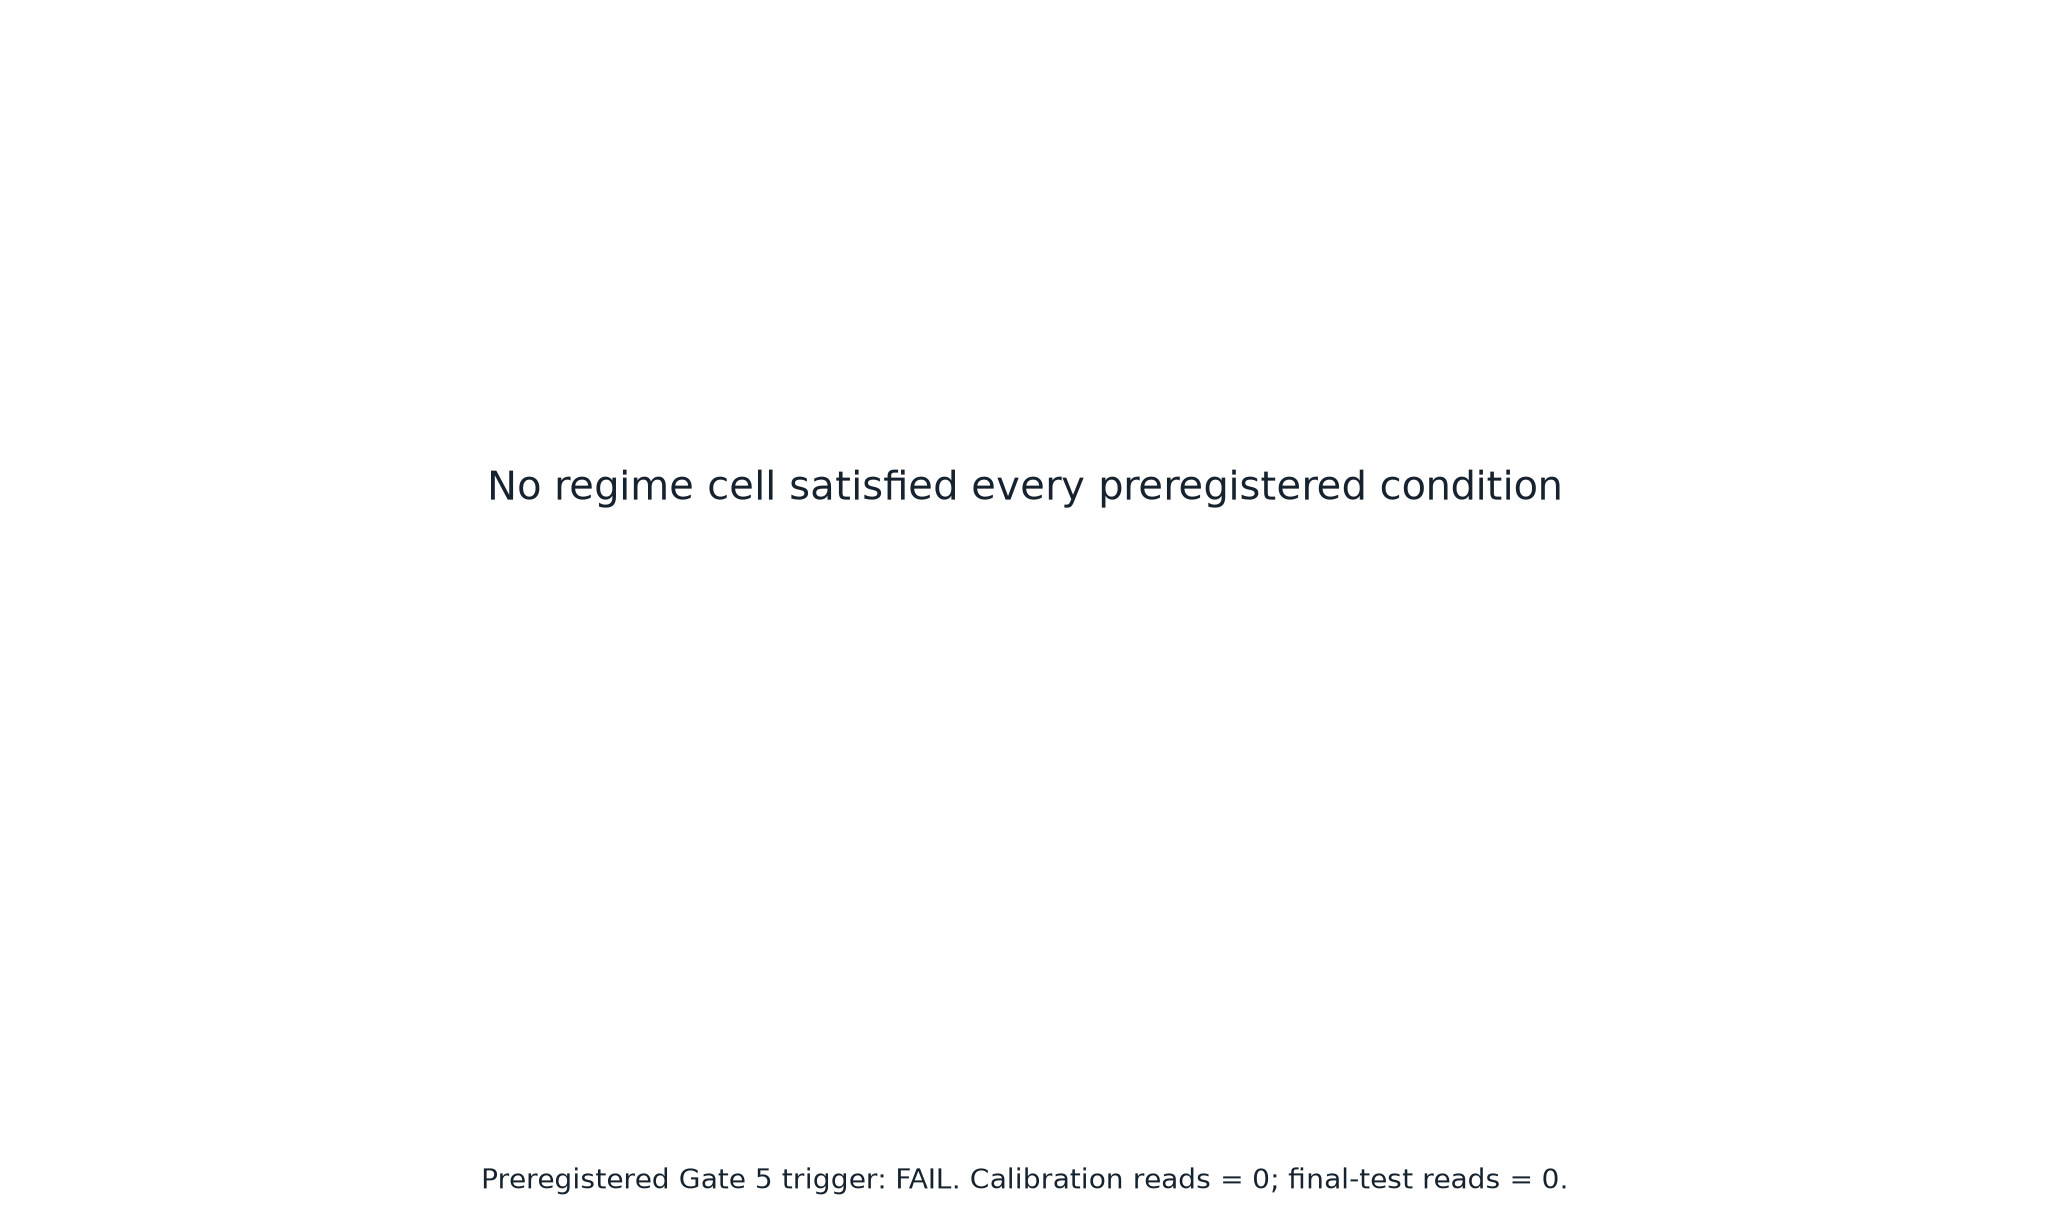
\includegraphics[width=0.92\textwidth]{figures/gate5_algorithm_trigger_regime_control.png}
\caption{Preregistered algorithm-trigger regime controls (RFIG-023). A
passing development trigger would have supported consideration of one further
algorithm study, not quantum advantage or operational deployment.}
\label{fig:gate5-trigger}
\end{figure}

Q02 and Q03 require a precise reading. They completed their authorized tasks,
but they did not satisfy the frozen eligibility condition for later rungs and
seed reruns. They are recorded as
\texttt{not\_reached\_under\_frozen\_eligibility}. Treating this state as a
failed experiment would overstate the evidence; treating it as an unreported
potential success would ignore the protocol. The paper reports the actual
decision state.

\begin{table}[t]
\caption{Primary and exploratory QML endpoints from the frozen evidence package. All values are development-only. Lower NRMSE and Brier score are better; higher recall is better for retaining actually feasible plans. The feasibility endpoint uses the fixed 0.5 threshold.}
\label{tab:gate5-results}
\centering
\footnotesize
\begin{tabularx}{\textwidth}{@{}>{\raggedright\arraybackslash}p{0.18\textwidth}>{\raggedright\arraybackslash}p{0.29\textwidth}Y@{}}
\toprule
Stage & Model and metric & Development result and meaning \\
\midrule
Primary Gate 5 & Fidelity quantum kernel (Q01); mean NRMSE & Q01: 0.646614; physics-residual C06: 0.008739. Protocol FAIL; no predefined subgroup passed. \\
Projected follow-up & Projected quantum kernel (Q01b; P001); mean NRMSE & Q01b: 0.661207; C06: 0.006833. Exploratory negative; about 97 times the C06 error. \\
Feasibility follow-up & Feasibility-only quantum kernel (FQK; P001); recall at 0.5 & Recall: 0.108860. It retained only 10.9\% of actually feasible cases, and classical controls were stronger. \\
Future lesson & Calibrated logistic model; feasible-case recall and Brier score & Recall: 0.804253; Brier: 0.142231. Protocol-design signal, not a safety result. \\
\bottomrule
\end{tabularx}
\end{table}


\subsection{Post-Gate 5 exploratory tracks}

Q01b tested whether changing the quantum readout while keeping the same
development discipline could materially alter the result. It did not. Q01b
attained mean NRMSE 0.661207, compared with 0.006833 for C06, a relative gap
of 95.77 times. Figure \ref{fig:q01b-curves} presents its learning curves
against the source-matched controls, while Fig. \ref{fig:q01b-geometry}
reports the projected-kernel geometry and dequantization diagnostics. These
are useful negative data: for this projected feature map, the representation
did not capture the residual structure better than the classical controls.
They do not establish that projected quantum kernels cannot work on any other
physical problem.

\begin{figure}[t]
\centering
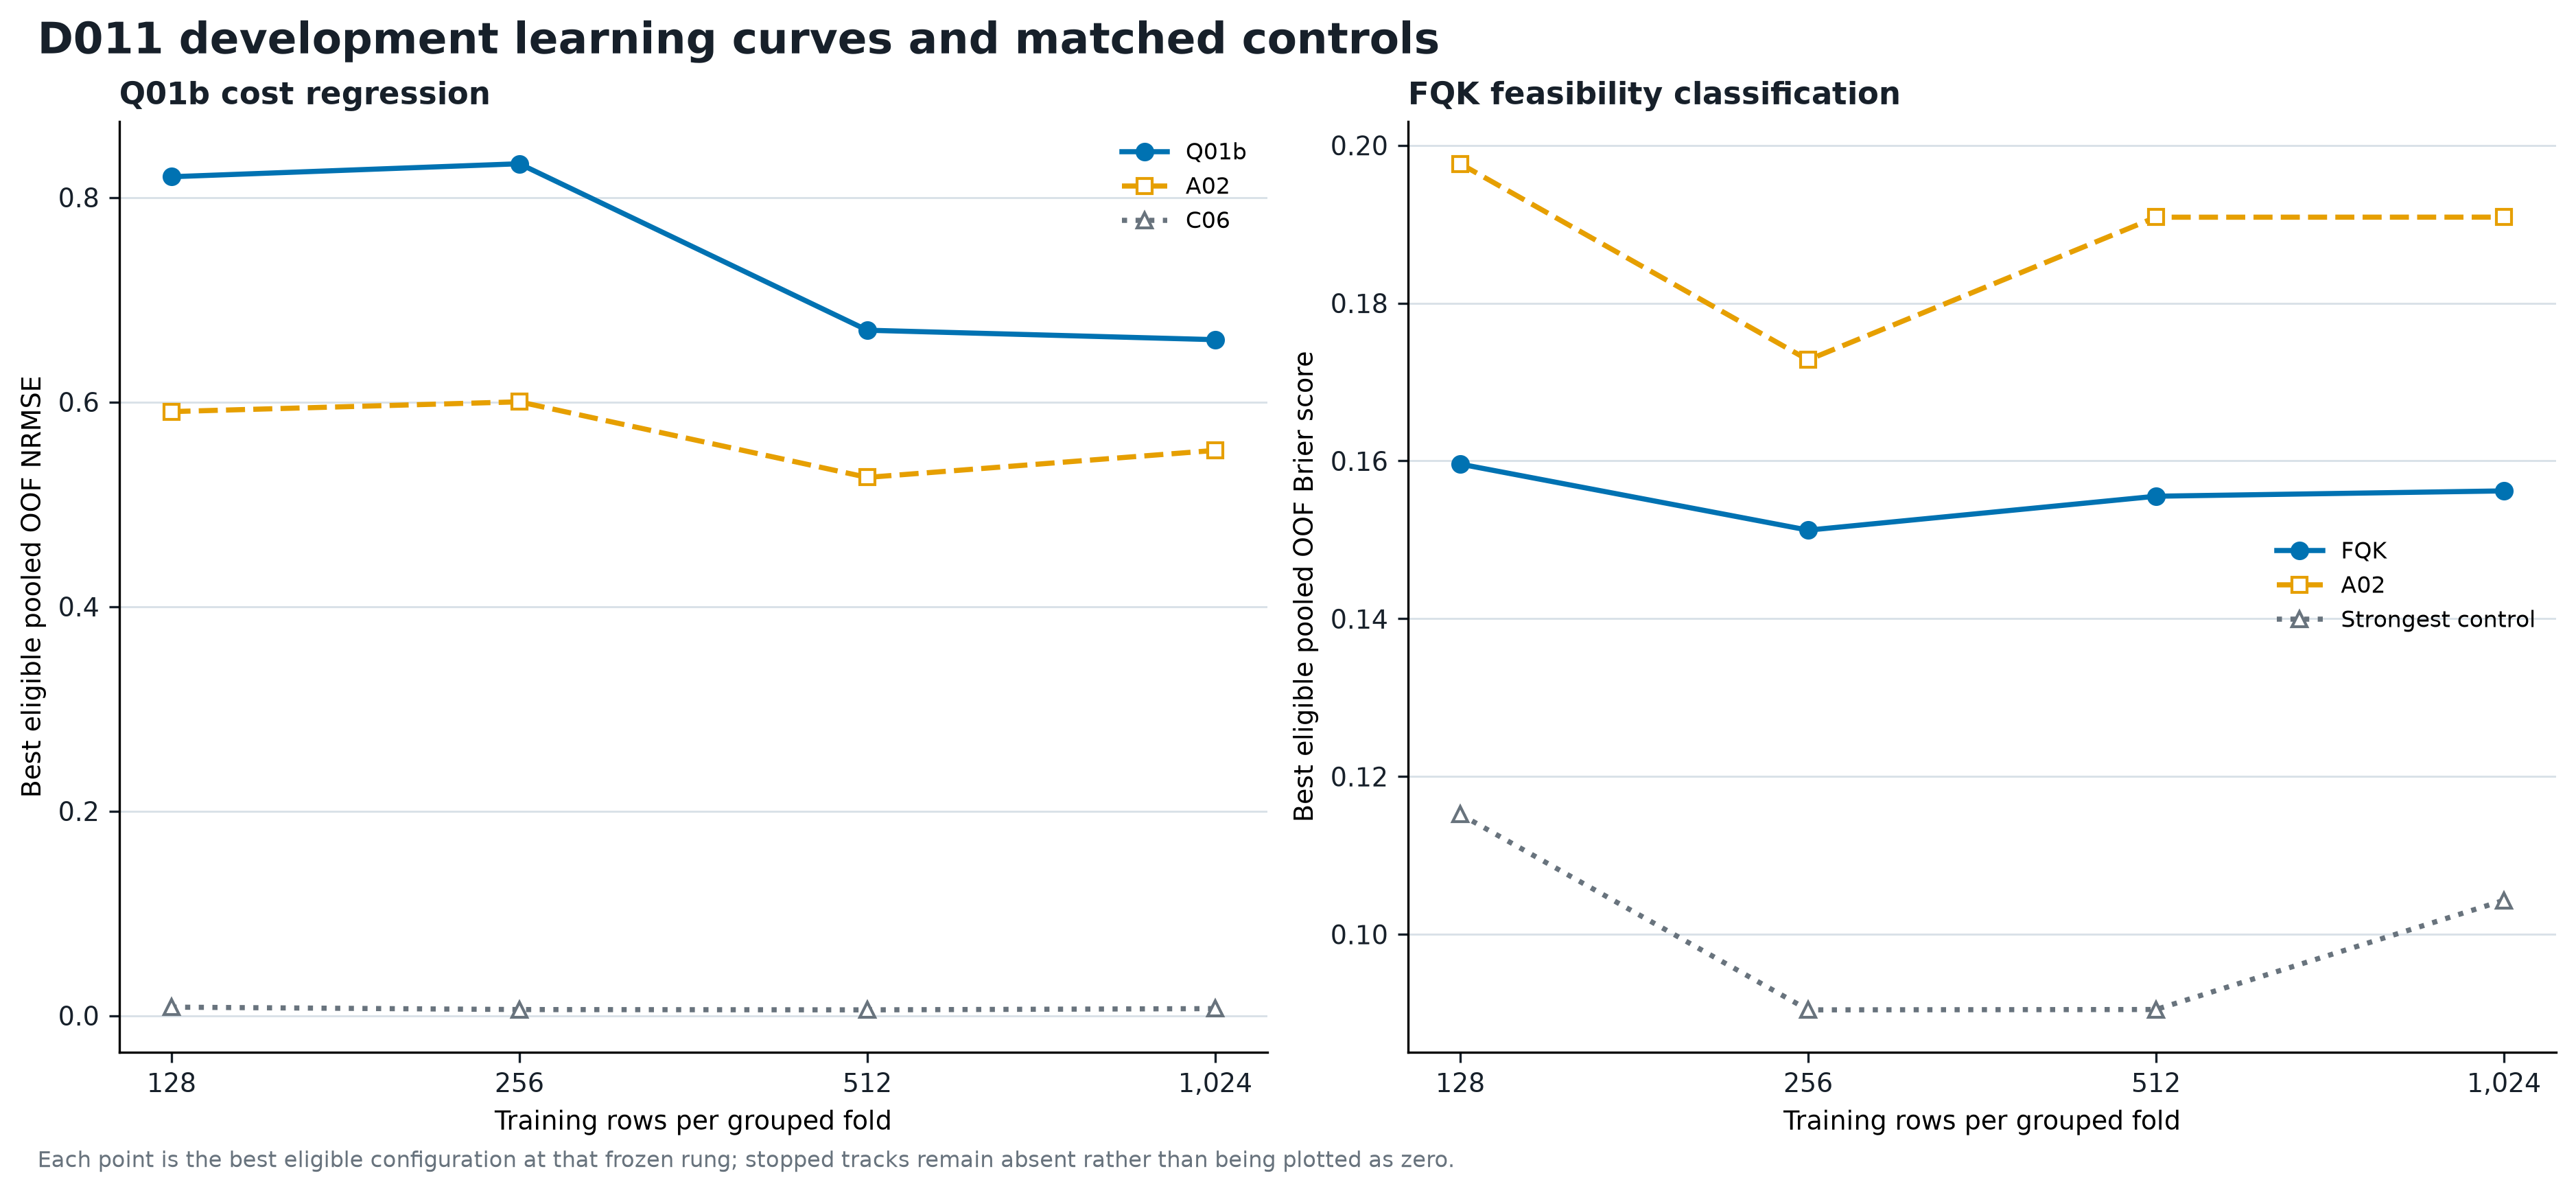
\includegraphics[width=\textwidth]{figures/post_gate5_d011_learning_curves.png}
\caption{D011/P001 projected-kernel learning curves and matched controls
(RFIG-026). The figure is development-only exploratory evidence and does not
revise the Gate 5 decision.}
\label{fig:q01b-curves}
\end{figure}

\begin{figure}[t]
\centering
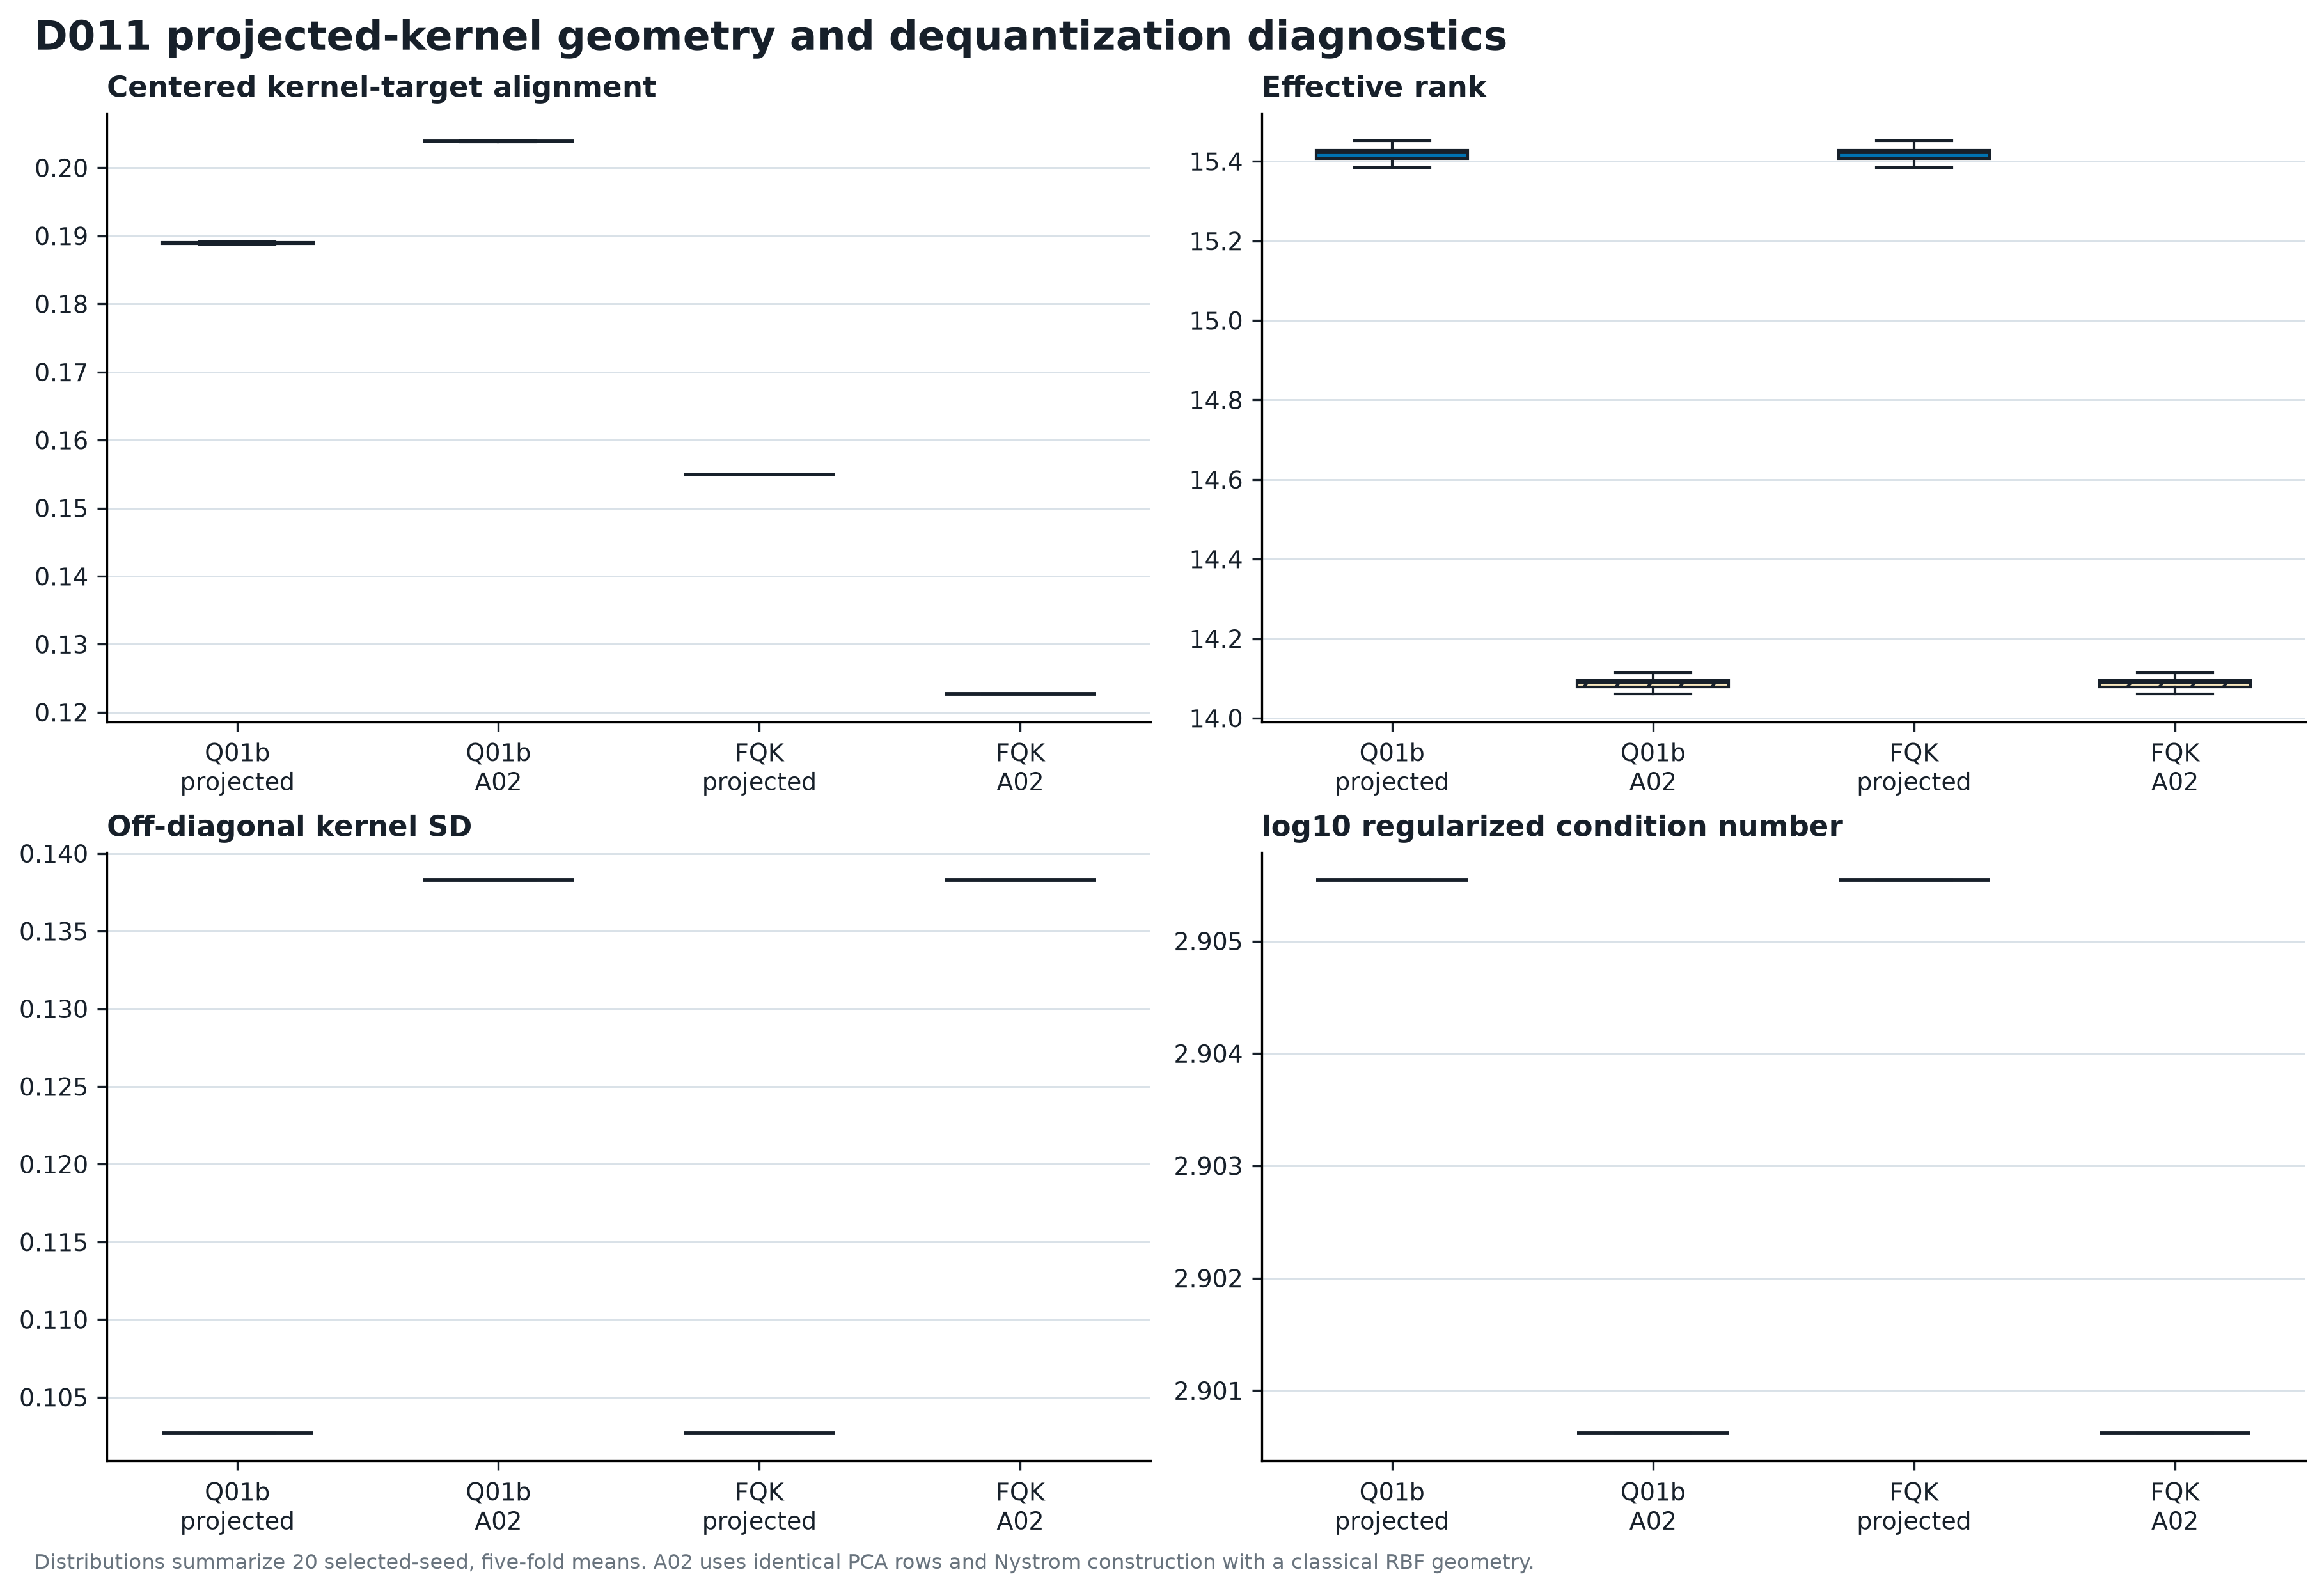
\includegraphics[width=\textwidth]{figures/post_gate5_d011_kernel_diagnostics.png}
\caption{Projected-kernel geometry and dequantization diagnostics (RFIG-027).
Selected projected kernels are compared with A02 classical RBF geometry on the
same fold-local PCA rows and Nystrom construction.}
\label{fig:q01b-geometry}
\end{figure}

The FQK classification track separates discrimination from a safety-filter
interpretation. It achieved AUROC 0.7436 and Brier score 0.1561, but recall at
the fixed threshold was only 0.1089. In a setting where missed unsafe cases
are material, the latter outcome prevents promotion to a safety-filter signal.
The endpoint plot in Fig. \ref{fig:fqk} makes this distinction visible. It is
not valid to call FQK useful for safety merely because one scalar metric is
above chance or because a quantum feature map was evaluated.

\begin{figure}[t]
\centering
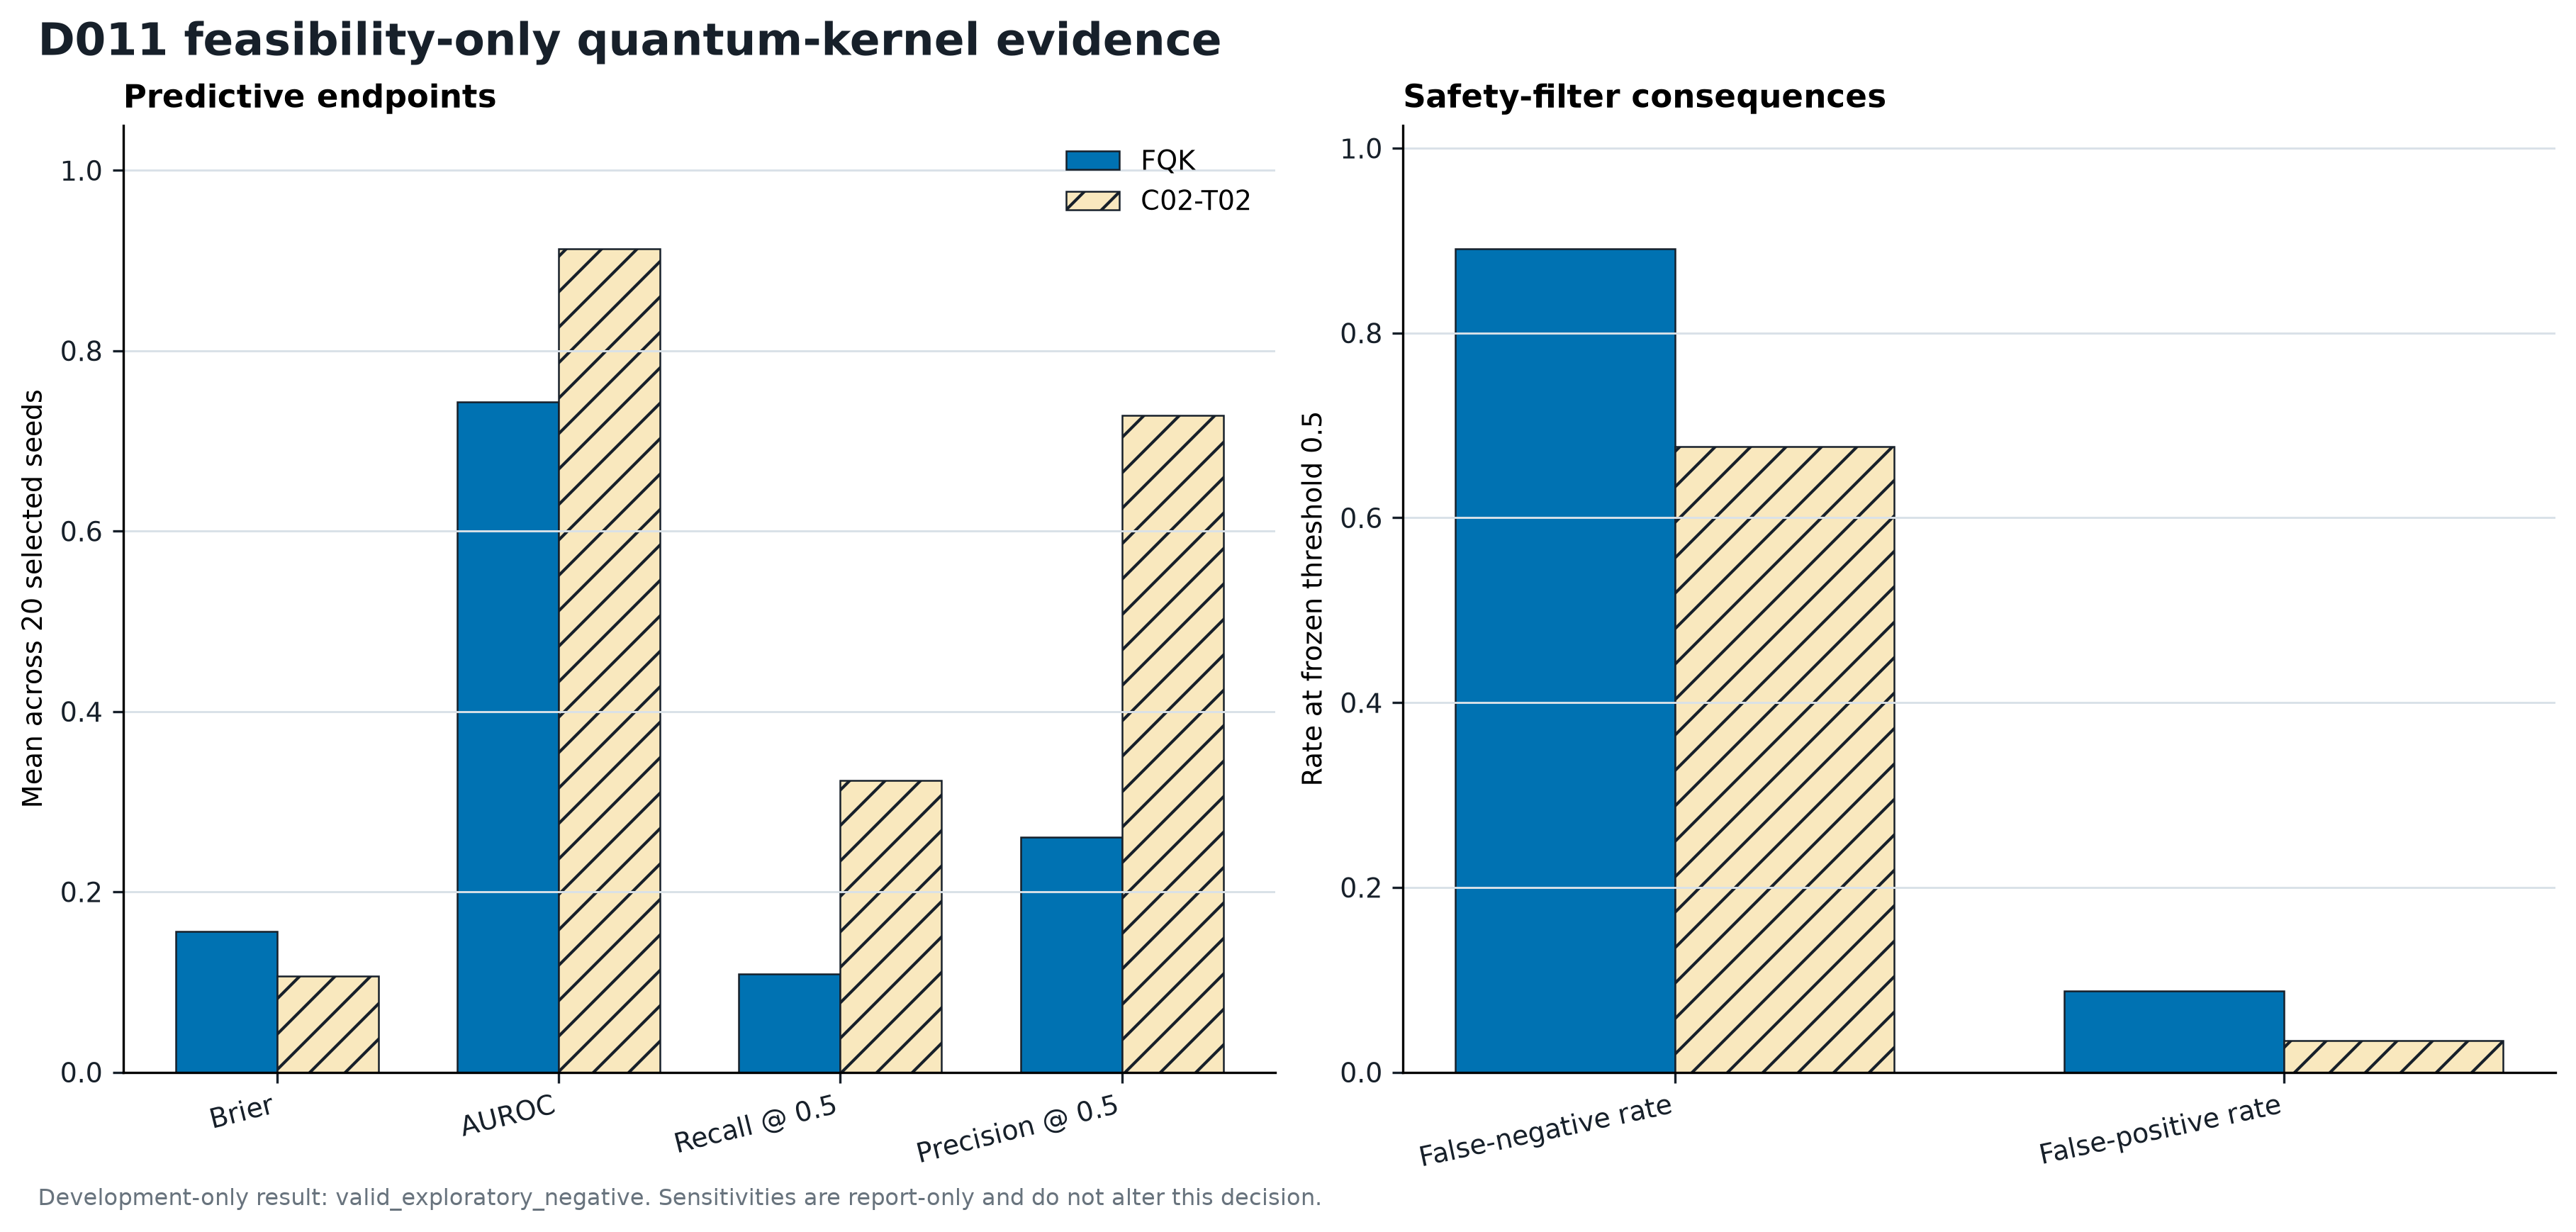
\includegraphics[width=\textwidth]{figures/post_gate5_d011_fqk_endpoints.png}
\caption{FQK predictive and safety-filter endpoints (RFIG-028). Brier,
discrimination, recall, precision, and consequence metrics are compared with
the strongest complete control. The frozen recall interpretation did not pass.}
\label{fig:fqk}
\end{figure}

The recall-first CSAFE-RF analysis provides a separate lesson for a future
protocol. A calibrated logistic model reached mean recall 0.804253 with
false-negative rate 0.195747 and Brier score 0.142231. That result identifies
an objective-design tension: a model selected only for calibration can miss an
unacceptable number of unsafe cases, whereas a future safety protocol should
prospectively define recall and calibration constraints together. CSAFE-RF was
not used to re-rank QML candidates, change a threshold, or authorize a mission
filter.

\subsection{Closed successor branch D034--D049}

The closed successor branch contains 16 prospectively bounded candidates. All
read the development scope only, used 39,000 development rows per campaign,
and completed with the recorded status
\texttt{complete\_valid\_negative}. The complete results are listed in Table
\ref{tab:successor-branch}. The table is intentionally included in full rather
than selecting only candidates with lower raw error than C06.

Several variants have a lower mean NRMSE than C06. This is a reason to inspect
the controls, not a reason to announce a quantum-specific result. The best raw
C06 comparison was D046, ORFRK-08-R2: NRMSE 0.0064363 versus 0.0068328 for
C06, an apparent 5.80\% reduction. Its matched second-stage RBF control,
TWO-RBF, attained 0.0067501. The candidate's improvement over that matched
classical alternative was therefore about 4.65\%, which is below the frozen
5\% branch-specific rule. The result does not meet the evidence standard for a
quantum-specific candidate.

\begin{figure}[t]
\centering
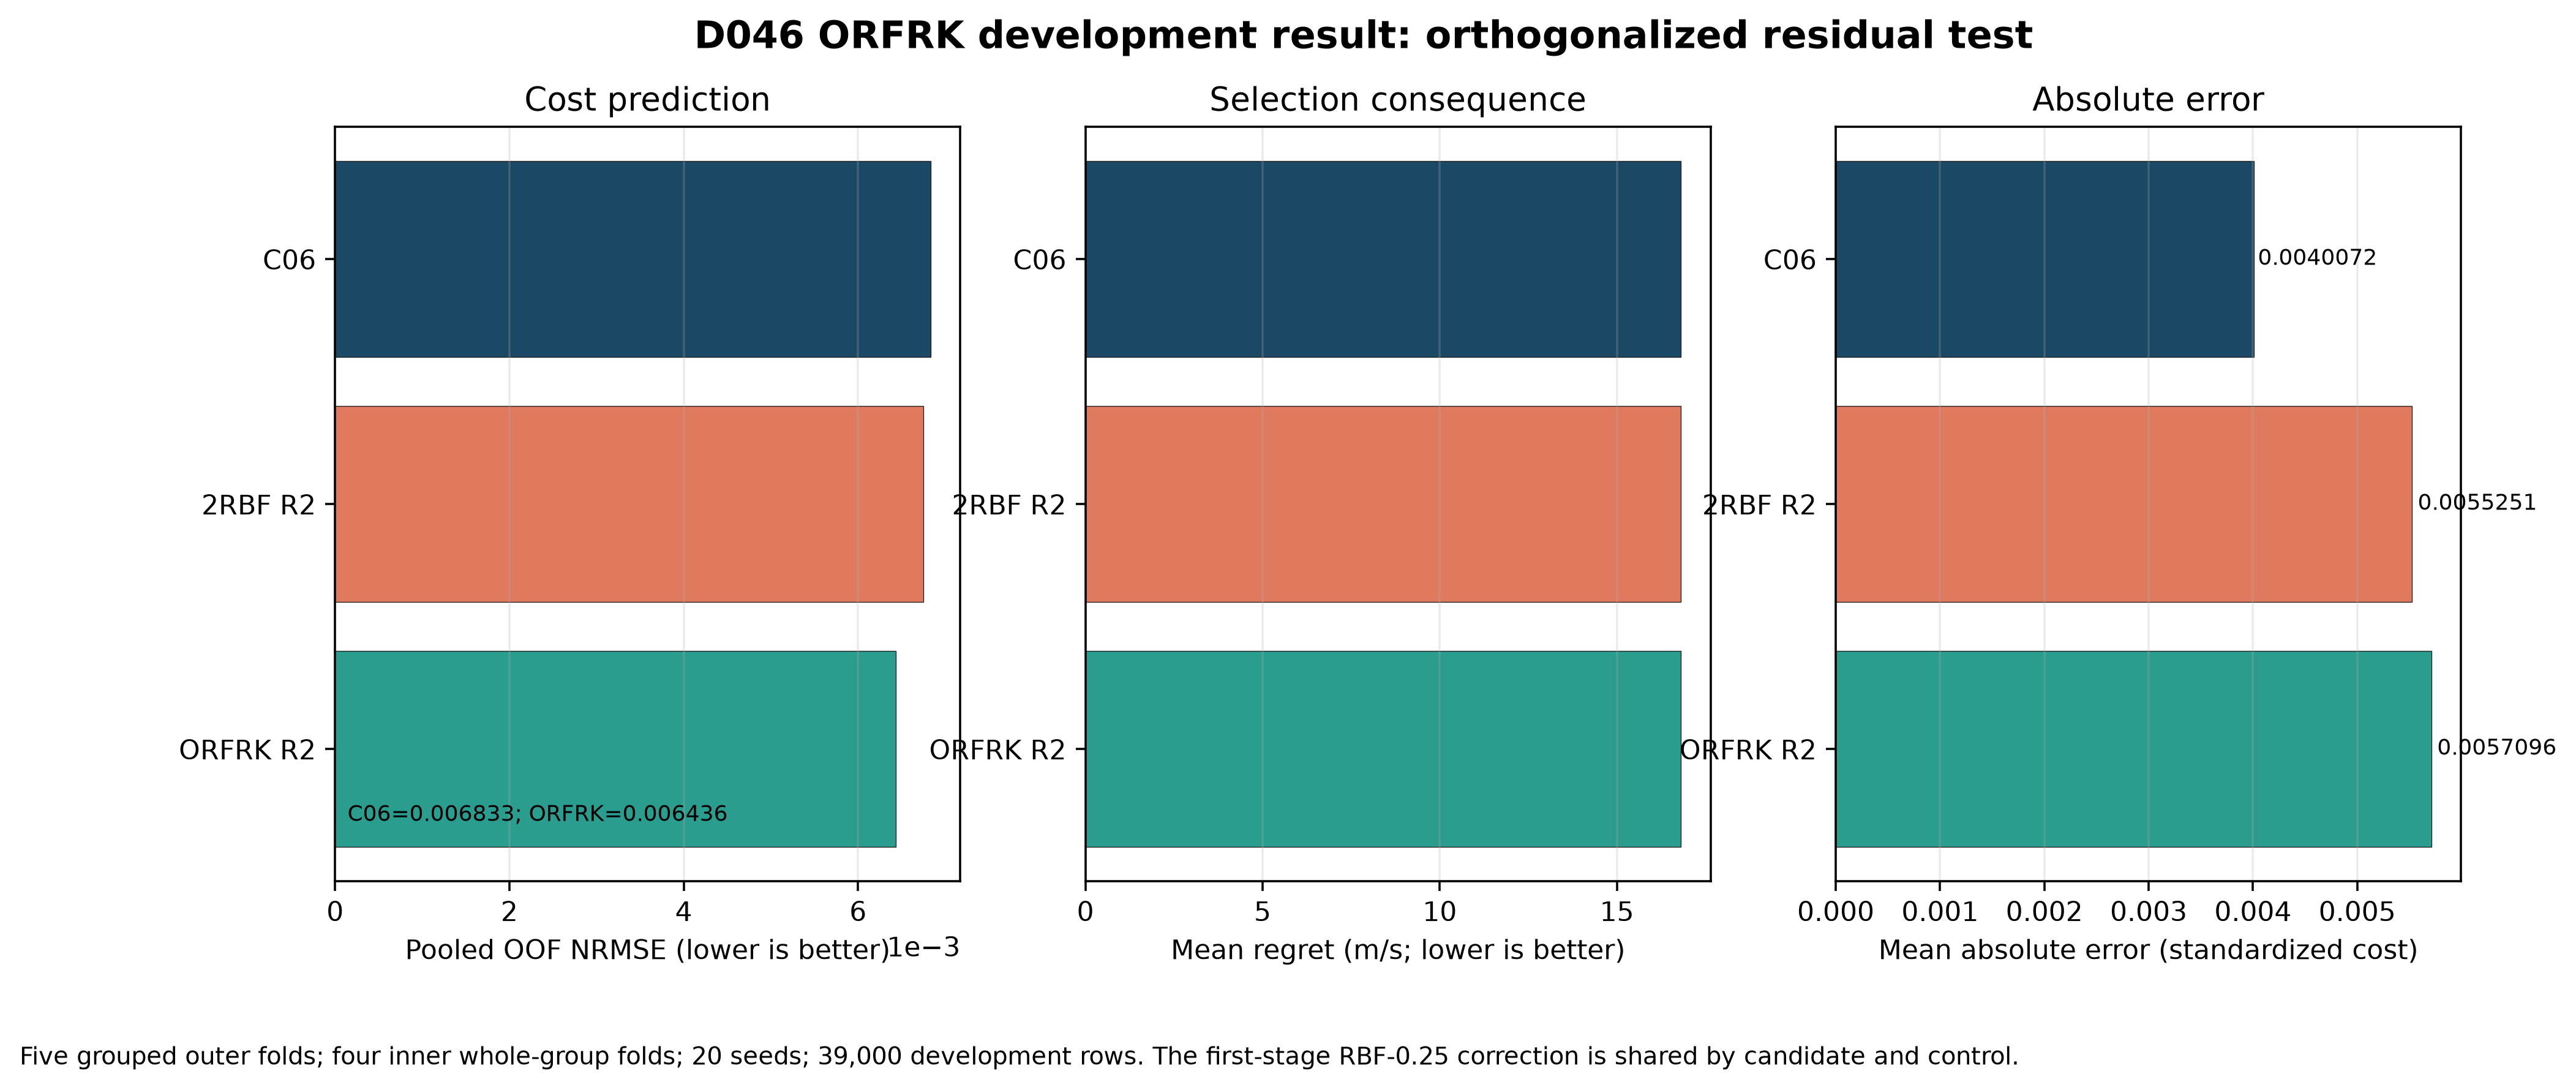
\includegraphics[width=\textwidth]{figures/post_gate5_d046_orfrk_result_comparison.png}
\caption{D046 ORFRK result comparison (RFIG-078). The q=8 candidate and a
matched second-stage RBF control are compared after a shared RBF-0.25
correction. Lower raw error than C06 is not sufficient for a QML claim.}
\label{fig:orfrk-result}
\end{figure}

\begin{figure}[t]
\centering
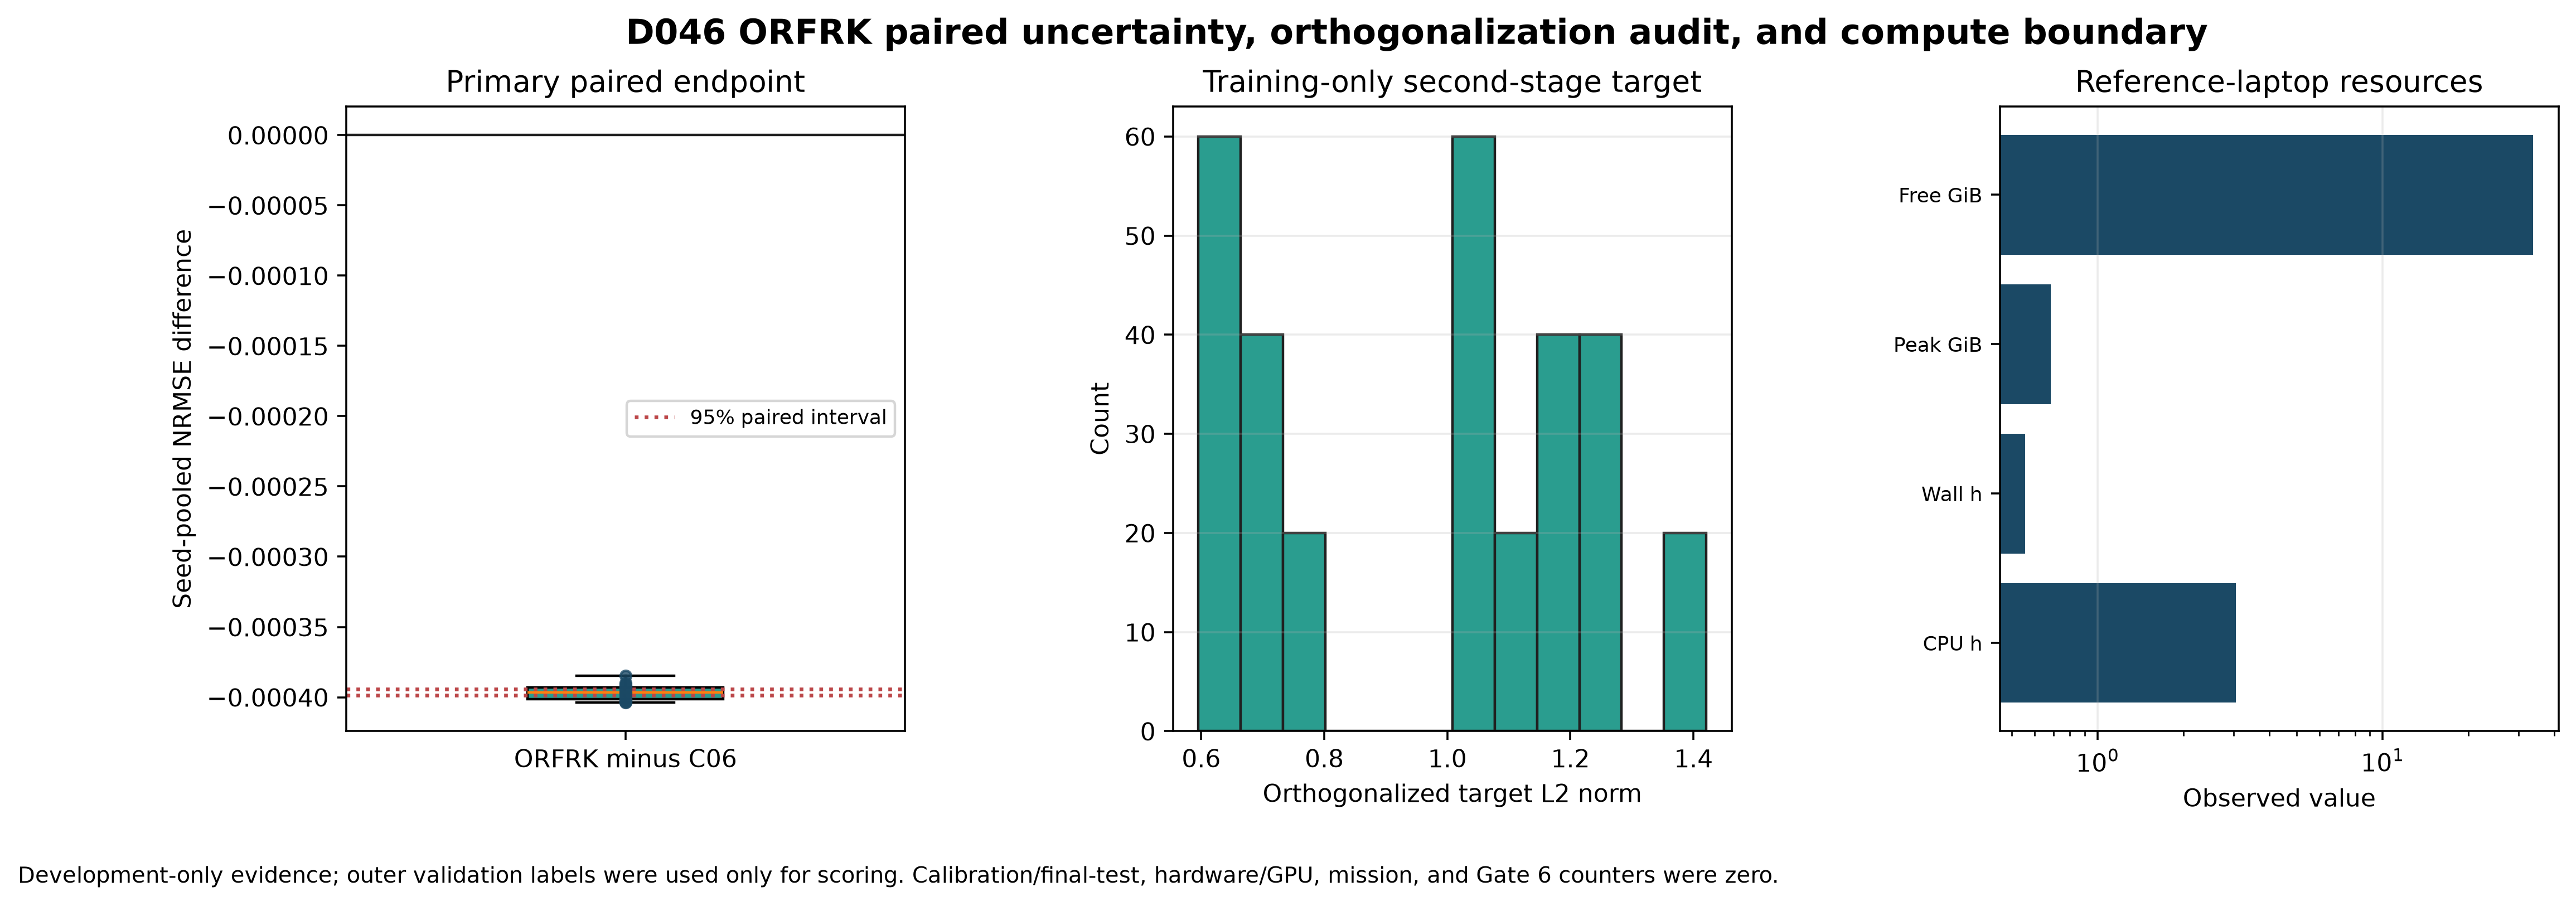
\includegraphics[width=\textwidth]{figures/post_gate5_d046_orfrk_audit_resources.png}
\caption{D046 paired audit and resource boundary (RFIG-079). The figure
reports the paired endpoint, training-only orthogonalization checks, integrity
evidence, and reference-laptop resources. It is not hardware or GPU evidence.}
\label{fig:orfrk-audit}
\end{figure}

\small
\begin{table}[!t]
\caption{Closed D034--D049 successor branch. Candidate names are immutable protocol IDs; their definitions are preserved in the repository. Every row is a valid development-only negative. The C06 NRMSE was 0.006833 throughout. Lower NRMSE is better, and a negative paired difference favors the candidate over C06, but each branch also had to pass its matched-control and stopping rules.}
\label{tab:successor-branch}
\centering
\scriptsize
\setlength{\tabcolsep}{2pt}
\renewcommand{\arraystretch}{0.92}
\begin{tabular}{@{}p{0.09\textwidth}p{0.24\textwidth}p{0.15\textwidth}p{0.17\textwidth}p{0.25\textwidth}@{}}
\toprule
Decision & Candidate & \shortstack[l]{Candidate\\NRMSE} & \shortstack[l]{Difference\\vs C06} & \shortstack[l]{95\% paired\\interval} \\
\midrule
D034 & PRQK-08-N & 0.029326 & 0.022493 & [0.022486, 0.022500] \\
D035 & CFQSR-08-N & 0.013463 & 0.006630 & [0.006627, 0.006632] \\
D036 & TAPQK-08 & 0.010382 & 0.003549 & [0.003547, 0.003551] \\
D037 & TSQR-08-L025 & 0.006848 & 0.000015 & [0.000015, 0.000015] \\
D038 & GFRK-08-L010 & 0.006647 & -0.000186 & [-0.000187, -0.000184] \\
D039 & EC-GFRK-08-L010 & 0.006466 & -0.000366 & [-0.000368, -0.000365] \\
D040 & CE-GFRK-08-L010 & 0.006504 & -0.000329 & [-0.000330, -0.000328] \\
D041 & HEFRK-08-E050 & 0.006592 & -0.000241 & [-0.000242, -0.000240] \\
D042 & AGEFRK-08-ADAPT & 0.006524 & -0.000309 & [-0.000310, -0.000308] \\
D043 & SFRK-08-CV & 0.006445 & -0.000387 & [-0.000389, -0.000386] \\
D044 & NIFRK-08-NL & 0.006751 & -0.000081 & [-0.000084, -0.000079] \\
D045 & MSFRK-ALL & 0.006731 & -0.000102 & [-0.000103, -0.000100] \\
D046 & ORFRK-08-R2 & 0.006436 & -0.000397 & [-0.000399, -0.000394] \\
D047 & OMFRK-ALL & 0.006952 & 0.000119 & [0.000113, 0.000125] \\
D048 & NSORFRK-08 & 0.006590 & -0.000243 & [-0.000244, -0.000242] \\
D049 & SSORFRK-08 & 0.006566 & -0.000266 & [-0.000268, -0.000265] \\
\bottomrule
\end{tabular}
\renewcommand{\arraystretch}{1}
\end{table}

\normalsize

\subsection{Evidence accounting and closure}

Evidence accounting confirms that the reported conclusion follows the
authorized boundary. D006 completed 871 of 871 tasks, with zero task failures
and zero reads of calibration or final-test data. The D011-R1 exploratory
campaign read 39,000 development rows and zero locked rows. No hardware
quantum job, mission-loop run, Gate 6 run, or final-test evaluation occurred.

Figure \ref{fig:closure} summarizes the closure recommendation. It reports
that no candidate is eligible for Gate 6; it does not represent an unexecuted
Gate 6 experiment. The experimental program was subsequently closed under
D055-C to permit publication preparation without turning future protocol ideas
into unapproved computation.

\begin{figure}[t]
\centering
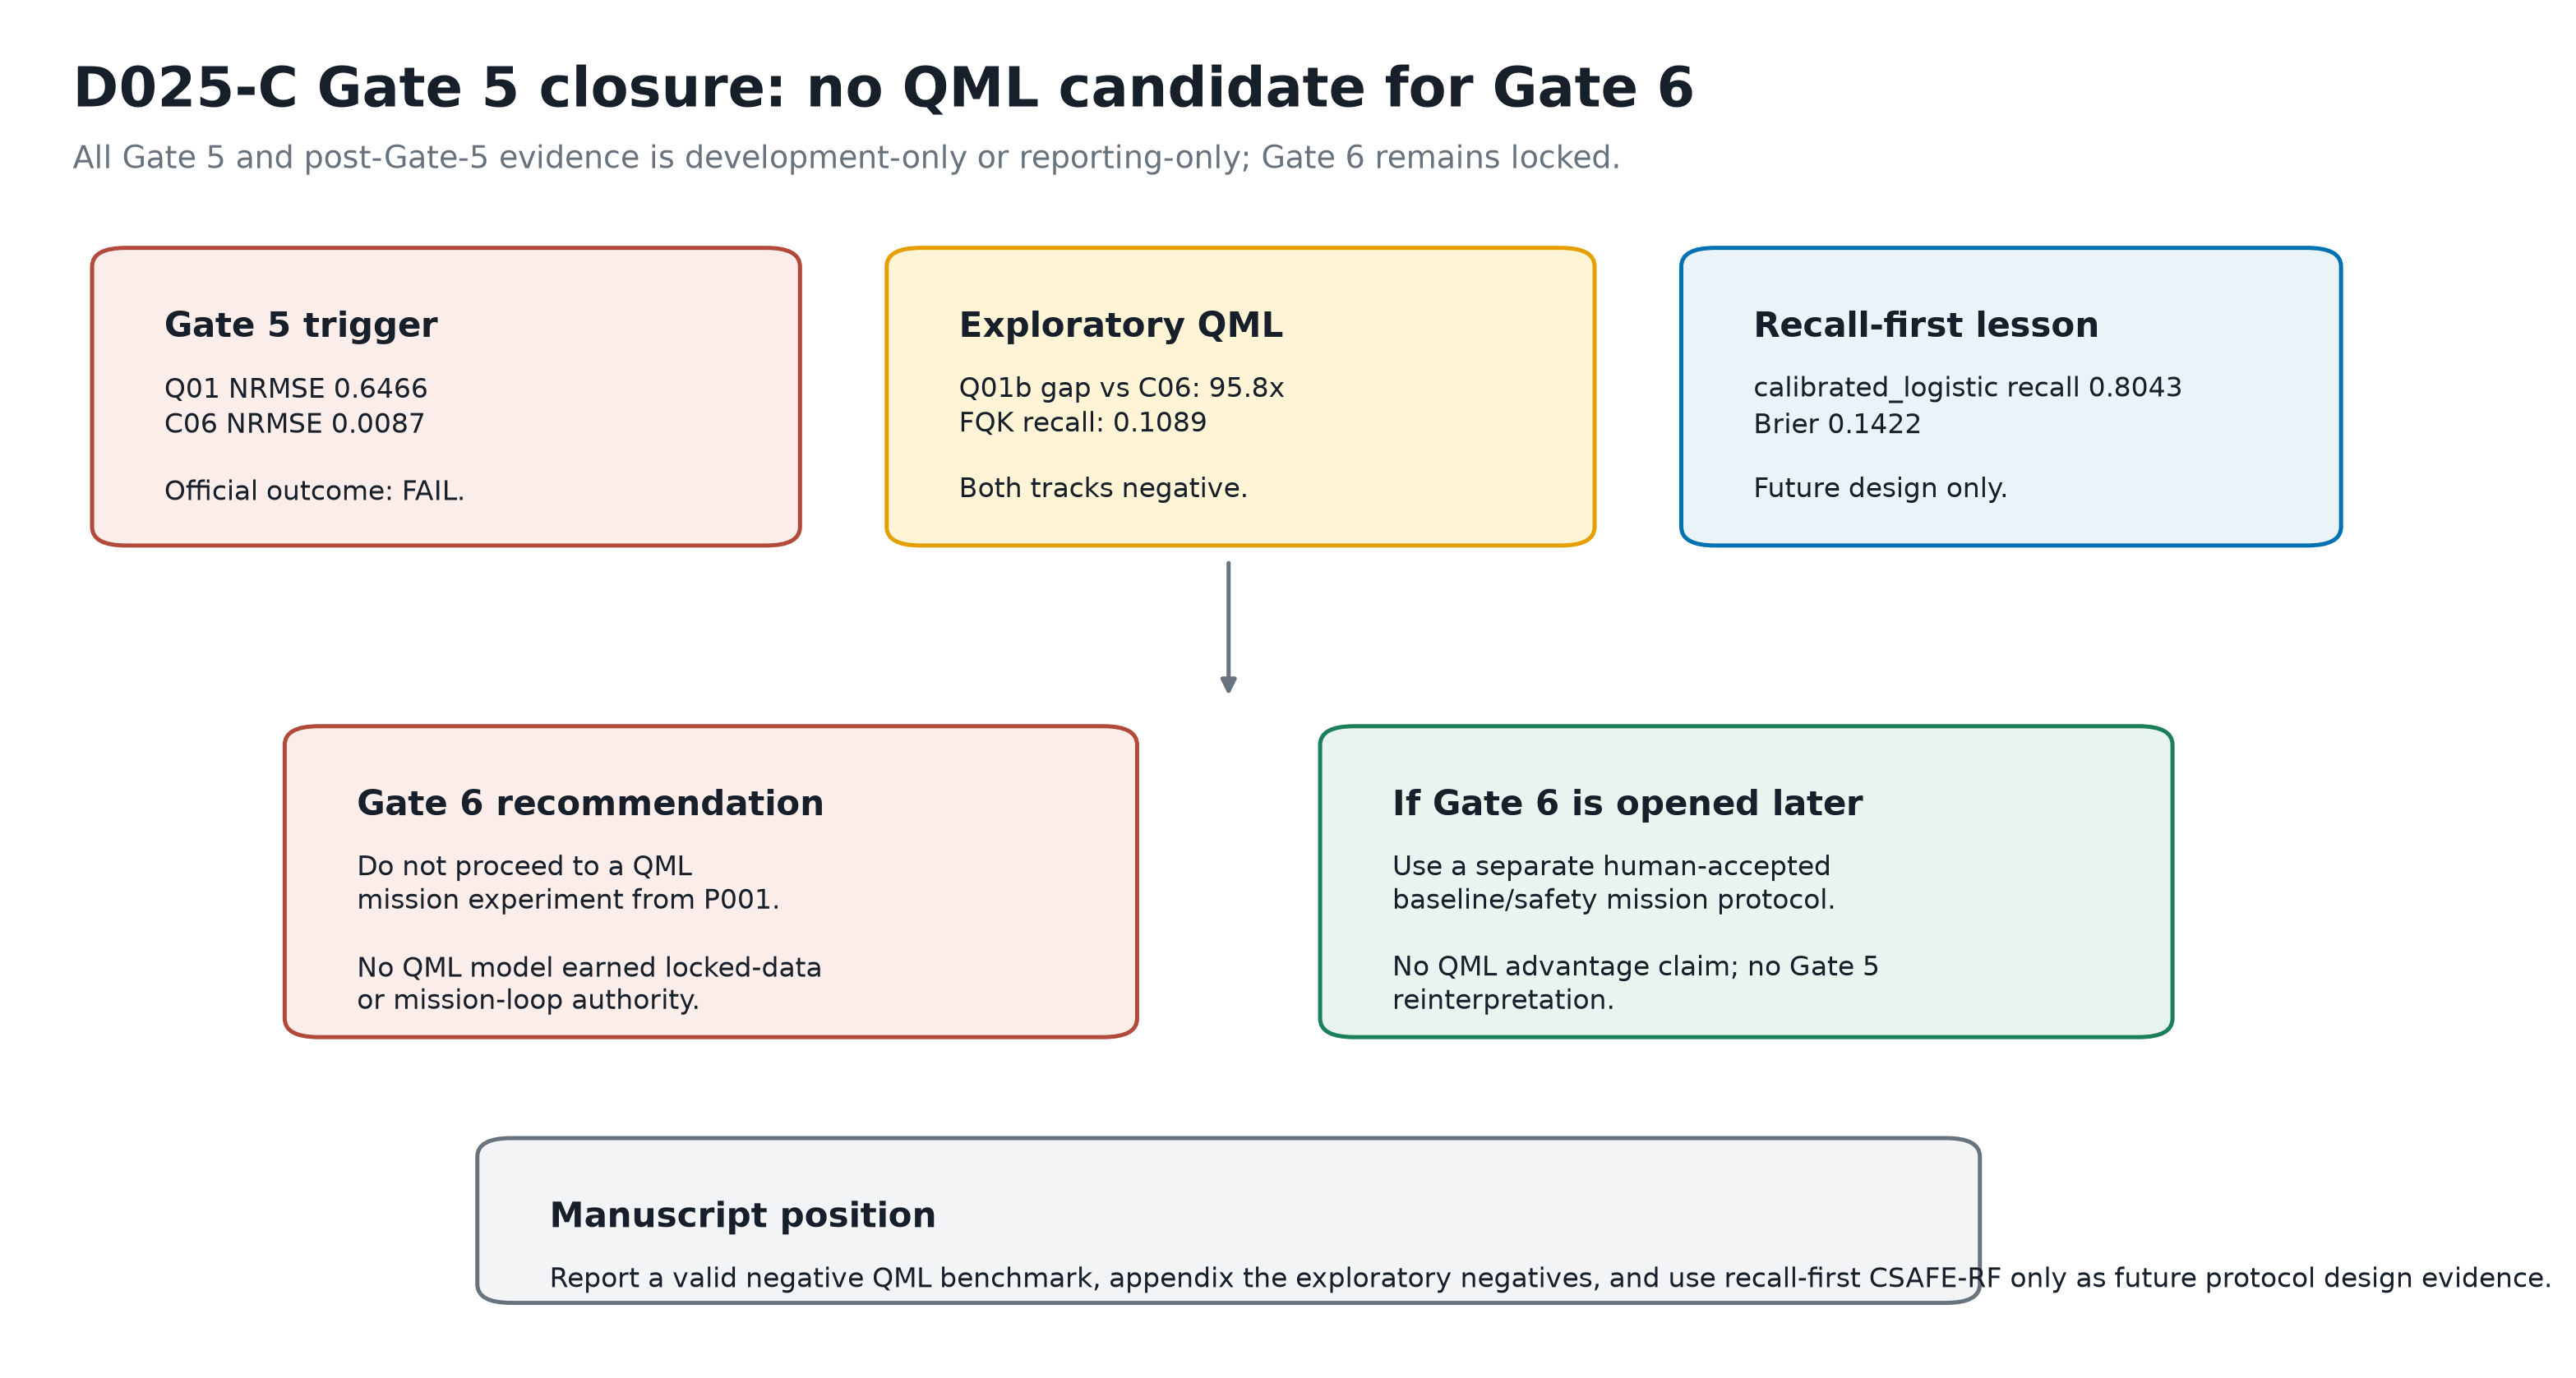
\includegraphics[width=\textwidth]{figures/post_gate5_d025_gate6_recommendation.png}
\caption{Gate 5 closure and Gate 6 recommendation (RFIG-044). No QML candidate
from the closed evidence branches is eligible for Gate 6. This is a closure
recommendation, not a Gate 6 result.}
\label{fig:closure}
\end{figure}

\section{Discussion}
\label{sec:discussion}

The principal finding is a controlled negative benchmark: the runs completed
validly, but the tested performance hypotheses were rejected. The Q01
fidelity-style quantum kernel was far behind the physics-residual control, and
the Q01b projected feature map did not close the gap. The feasibility-only
kernel did not meet its fixed multi-metric screening criteria. The successor
branch demonstrates an additional failure mode that matters beyond this task: a
candidate can improve over one baseline yet fail against a classical model with
the same staged construction. That distinction is why matched dequantization
controls and thresholds fixed before outcomes belong in the protocol.

The result is scientifically useful because the negative conclusion is
specific. It rules out a family of tested feature maps and successor
constructions under a particular public-data scenario generator, grouped
development procedure, resource envelope, and comparator set. It does not
rule out all QML, all cislunar machine learning, or all future quantum
hardware. Such broad claims would require evidence absent here, including
separate tasks, new preregistration, scalability studies, noise analysis,
hardware measurements, and appropriate classical resource comparisons.

The physics-residual control is a key methodological result. A generic
classical baseline is not sufficient when the prediction target contains
structure that a low-fidelity model can represent directly. C06's performance
shows that, for this benchmark, the available physical residual structure is
more informative than the tested quantum fidelity features. That observation
does not establish a theorem about quantum circuits; it establishes a
task-specific comparison of inductive bias, the kinds of patterns each model is
built to represent, that future proposals must beat fairly.

The retained Q02/Q03 status also matters. Many reports collapse all
non-advancing paths into a single ``failure'' category. Here, the first-rung
tasks ran correctly, but the candidates were ineligible for larger-rung
computation under a rule frozen before results. Keeping
\texttt{not\_reached\_under\_frozen\_eligibility} separate from a task failure
makes the evidence ledger more truthful and prevents a later analyst from
inventing a selection path that never existed.

The paper's societal relevance is therefore not a claim of operational benefit.
It is a reusable, human-centered research pattern for high-consequence AI:
include an eligible simulator-validation scope, freeze data transformations and
groups, use a physics-aware control, compare against matched classical
alternatives, retain null outcomes, and make the claim boundary checkable from
source artifacts. This helps researchers, reviewers, and future decision-tool
designers distinguish a reproducible negative result from evidence for
automation. Its value is in reducing the risk that an exciting but unsupported
model claim is presented as a safe decision-support capability.

The HCI implication is deliberately limited. The present results do not show
that a planner would understand, trust, reject, or use the evidence package
well. They specify what a later human-centered evaluation should not omit:
provenance, model scope, uncertainty, failure visibility, and a non-automated
fallback. Testing those requirements with intended users remains future work.

\subsection{Implications for QML benchmarking}

The QML literature has repeatedly shown that benchmark conclusions depend on
which classical methods are made available to the comparison
\cite{bowles2024,schnabel2024}. The D046 result gives a concrete trajectory
application example. Comparing only with C06 would make the candidate's raw
5.80\% difference look promising. The matched TWO-RBF alternative explains
enough of that difference that the candidate fails the frozen 5\% rule. The
interpretation changes because the question changes from ``is the candidate
better than one baseline?'' to ``is its incremental mechanism still supported
when a classical model is given the same residual construction?''

This contrast does not show that the matched control is the universally best
classical model. It shows why a QML result needs multiple controls chosen to
test the claimed mechanism. A fair comparison is not one that intentionally
makes every model identical; it is one that removes alternative explanations
for the purported QML contribution. In this benchmark, the alternative
explanation was a classical residual representation, and it remained
competitive.

\subsection{Safety objective as a distinct scientific question}

The FQK and CSAFE-RF records demonstrate that predictive metrics must be tied
to both label meaning and intended action. In these executed analyses, the
positive label is feasible. AUROC measures overall ranking, Brier score measures
probability error, and recall measures how many actually feasible options are
retained. Precision and the false-positive rate address the different risk of
admitting an actually infeasible option. FQK remains negative under its frozen
multi-metric rule even though its AUROC is above random, because its Brier score
and feasible-case recall did not match the classical controls. This guards
against promoting a model by whichever metric looks most favorable afterward.

The higher-recall classical result is not a rescue or a safety result. It is a
future design lesson: a screening protocol should define, before fitting, a
minimum feasible-case recall for usefulness, a maximum infeasible-case
false-positive rate for protection, a calibration requirement, and the action
taken when the model abstains. Those quantities cannot be replaced by a single
``safety'' score. Testing such a policy requires a separately authorized
experiment; using it to alter Gate 5 after inspection would invalidate the
original test.

\section{Limitations and Threats to Validity}
\label{sec:limitations}

First, the study is public-data and development-only. Calibration and
final-test data were not read. The paper cannot estimate final-test error,
operational calibration, mission-loop behavior, propellant savings, or flight
readiness. The use of Artemis-related public work establishes relevance of the
problem framing, not access to mission-owned truth data or authority to draw
mission conclusions.

Second, simulator agreement is bounded. The Gate 3 results support the
eligible public endpoint comparisons, but they do not validate every force
model, contingency, navigation product, or human-rating consideration. RTC3
is source-ineligible, and some generated scenario decisions do not have an
independently feasible numerical reference. Those limitations remain in the
dataset rather than being removed after model results are observed.

Third, the quantum experiments are small-qubit classical statevector
simulations within a laptop-bounded resource envelope. They do not report shot
noise, gate noise, device connectivity, state-preparation latency,
transpilation cost, hardware calibration, or end-to-end quantum runtime. They
cannot demonstrate quantum speedup, hardware efficiency, or a practical
quantum advantage. An alleged advantage would require all of those questions
to be addressed against a fair classical resource baseline.

Fourth, the methods are limited by their frozen design. The chosen
preprocessing, feature maps, sample rungs, controls, and thresholds make the
comparison interpretable but restrict the scope of inference. A different
method can be scientifically tested only through a new protocol, not by
modifying the completed campaign until a favorable result appears.

Finally, the literature synthesis is bounded, not systematic. The inclusion
set provides methodological context and control requirements but does not
prove that no related method exists. This is why the paper makes a benchmark
claim rather than a novelty or universal-performance claim.

\section{Future Research Boundary}

The negative results motivate questions about task-specific symmetry,
representation, and residual structure, but the completed evidence does not
answer them. A future geometric-QML direction was discussed as a hypothesis,
not as a result. Here a symmetry would be a transformation, such as rotating
all relevant vectors together, that preserves the physical relationship between
inputs and labels. An equivariant model is designed so that its output changes
consistently under such a transformation. The first unanswered question is
whether any nontrivial symmetry actually survives fixed Earth--Moon--Sun
ephemerides, thrust constraints, and reference-frame choices. Equivariance
alone would not imply a QML advantage over classical equivariant models.

A future protocol would require a mathematical contract, a symmetry audit,
baseline reproduction, a representation- and parameter-matched classical
comparison, ablations of symmetry and initialization, resource accounting,
and explicit rejection criteria. The D054-A/P018 binding freeze records how a
future audit could specify its representation, dynamical Lie algebra (DLA)
basis, allowed circuit generators, development-only case groups, numerical
tolerance, output paths, and figures. A DLA describes the transformations that
can be generated by the allowed circuit operations. Closure decision D055-C
declined to execute the audit. Accordingly, this manuscript contains no
DOP853 trajectory replay (a high-order numerical integration check), no
singular-value-decomposition (SVD) rank or nullspace result, no new symmetry
dataset, no variational circuit training, and no geometric-QML performance
claim.

This boundary is not a weakness in reporting. It prevents a promising idea
from being laundered into evidence through narrative. The appropriate next
step, if future authors choose to reopen research, is a separately approved
protocol that can reject the hypothesis as readily as it can support it.

\section{Data, Code, and Figure Availability}

The source repository, governance records, machine-readable reporting outputs,
figure registry, and the published source release are available at
\href{https://github.com/taechasith/QMLforArtemisIV}{the project repository}.
The published release record is
\href{https://github.com/taechasith/QMLforArtemisIV/releases/tag/v0.3.0}{release v0.3.0}.
This paper package copies the exact figures used in the manuscript and the
three core result tables plus figure registry. The package does not include
calibration or final-test rows, mission-owned evidence, trained weights, or
unexecuted future-protocol outputs.

\section{Conclusion}

Under the frozen public-data development benchmark, the tested QML candidates
did not outperform strong classical controls, and no tested candidate is
eligible for a Gate 6 mission experiment. The primary whole-state fidelity
kernel (Q01), projected-kernel follow-up (Q01b), feasibility-only kernel (FQK),
and all 16 bounded successors produced negative outcomes under their stated
criteria. The strongest successor appeared better than the C06 physics-residual
control, but its advantage over a like-for-like classical alternative was only
4.65\%, below the 5\% threshold fixed before execution.

The study's contribution is a reproducible negative result with an explicit
governance and human-centered claim structure. It reports what was tested, what
did not advance, what remains a future lesson, and what a human reviewer would
need to see before considering further authorization. Its practical societal
value is a more accountable way to evaluate AI evidence for high-consequence
decision contexts, not a deployed mission capability. It does not establish
quantum advantage, fuel savings, mission utility, hardware performance, flight
readiness, NASA approval, or an invented QML model. That restraint is necessary
for the result to be useful.


\begin{credits}
\subsubsection{\ackname}
Reserved for an advisor contribution statement, pending advisor review.
\end{credits}

\appendix
\section*{Appendix: Reproducibility and Evidence Ledger}

The paper package is structured so that a reviewer can trace every main-text
number to a copied source table or figure. The Gate 5 CSV and the successor
branch-summary CSV (comma-separated-value) files in
\texttt{results\_tables/} provide the numerical values
reported in Tables \ref{tab:gate5-results} and \ref{tab:successor-branch}.
The copied figure registry records the title, evidence status, source data,
generator, digest, and claim boundary for every figure included here. The
figures retain their registry identifiers in their captions.

The release package provides scripts, fixed configuration records, data cards,
and decision logs. Reproduction of the published development
figures should begin from the tagged repository state and should preserve the
lock on calibration and final-test data. Re-running a report-generation script
is different from authorizing new fitting or a new experimental campaign.

\subsection*{Interpretation Checklist for Reviewers}

The following checklist summarizes the intended reading of the paper:
\begin{enumerate}
\item Treat Gate 3 as an eligible-scope simulator consistency result, not a
mission validation result.
\item Treat Gate 5 as rejection of the Q01 fidelity-kernel hypothesis on this
development benchmark, not a universal statement that QML cannot work.
\item Treat the projected Q01b kernel, feasibility-only FQK classifier, and 16
successors D034--D049 as development-only negative evidence that cannot revise
Gate 5 or open Gate 6.
\item Treat D046 as evidence that an apparent improvement over the C06
physics-residual model must also be tested against a like-for-like classical
control.
\item Treat the recall-first analysis as a future lesson about retaining
feasible plans while controlling infeasible admissions, not as a deployed
safety filter.
\item Do not infer quantum advantage, hardware performance, propellant saving,
or flight readiness from any figure or table in this package.
\end{enumerate}

\subsection*{Literature-Source Audit}

The literature review was re-audited against the completed experiment. The
repository extraction matrix retains 23 accepted records, the random-Fourier
source behind A01, and the quantum-kernel benchmark source used in the P001
discussion. Mission, simulation, classical-trajectory, QML-method, and
benchmarking sources justify the task, controls, and claim boundary; the
quantum-annealing source is adjacent context and remains excluded from the QML
candidate set. The bibliography contains only sources supporting an explicit
statement, design choice, control, or scope decision. The full role-by-source
matrix remains in \texttt{tables/literature\_source\_audit.tex}.

This audit does not turn prior literature into evidence for the present models.
Variational QML, quantum reinforcement learning, and quantum annealing are
cited to explain why model families were frozen, controlled, or excluded. The
empirical findings remain those from the registered public-data development
campaigns reported here.


\bibliographystyle{splncs04}
\bibliography{references}

\end{document}
